\chapter{Assessing the agro-hydrological impact of climate and agricultural management changes using AquaCrop-Hydro}\label{ch:achtoep}
\chaptermark{Agro-hydrological impact analysis}
%This chapter is based on word document of 5-4-2016

\section{Introduction}
The AquaCrop-Hydro model was developed to fill the need for a parsimonious agro-hydrological model, with low data and calibration requirements, that can be used to study the impact of agronomic and environmental changes on both crop productivity and catchment hydrology. Model evaluation in \autoref{ch:aquacrophydro} showed that AquaCrop-Hydro, being a combination of AquaCrop and a conceptual hydrological model, performed well to simulate crop productivity and runoff at the catchment outlet of an agricultural catchment in Belgium. 

Because of its process based nature and its good balance between model accuracy and data requirements, AquaCrop-Hydro has many advantages to study the agro-hydrological impact of climate or agronomic management changes.  Unlike conceptual hydrological models, AquaCrop-Hydro can simulate the effect of agricultural management on catchment hydrology. In addition, the effect of climate change is simulated more dynamically as its effect on crop growth and transpiration is taken into consideration for simulation of the soil water balance. Furthermore, AquaCrop-Hydro has relatively low computational requirements. This is especially useful for climate change impact assessment, which  typically requires a large number of simulations for a large ensemble of climate models to consider the high uncertainty in future climate projections \parencite{collins2007}. 

Yet, these many advantages for agro-hydrological impact assessment have never been demonstrated. For that reason, this study evaluates the use of AquaCrop-Hydro for investigation of the impact of climatic and agronomic management changes on crop development and crop productivity as well as catchment hydrology for an agricultural catchment in Belgium.

\section{Methodology}
\subsection{Study area}
The catchment of the Plankbeek stream, located in the sandy loam region of Flanders (Belgium), covers an area of \SI{4.5}{km^2} and ranges in altitude between 17 and 70 m a.s.l. On the silt loam to sandy loam soils of the catchment, agricultural land use dominates (94\% of catchment area). In addition to grassland (18\% of  agricultural land), the most prevalent crops are winter wheat (20\%), potato (16\%), maize (14\%), sugar beet (11\%) and peas (6\%) \parencite{agiv2014, agiv2001, vlm2014}. The area is characterised by a temperate climate with mild winters and cool summers, with rainfall uniformly spread throughout the year. More details on the study area are presented in \autoref{ch:aquacrophydro}.

\subsection{The AquaCrop-Hydro model}
The agro-hydrological model AquaCrop-Hydro was developed as a combination of the AquaCrop crop water productivity model \parencite{hsiao2009,steduto2009,raes2009a,vanuytrecht2014a} and a lumped conceptual hydrological model per the generalized structure by \textcite{willems2014}. AquaCrop-Hydro simulates the daily soil water balance, crop development and production, based on limited inputs of climate data (daily rainfall, reference evapotranspiration (\ETo), minimum and maximum temperature and global average annual \COtwo concentration \COtwocon), crop characteristics (e.g. sowing date, length of the growing period, harvest index, rooting depth, sensitivity to abiotic stresses), soil and groundwater table characteristics (soil water retention characteristics and saturated hydraulic conductivity, groundwater table depth), and agricultural management practices for each land unit of the catchment. Based on few hydrological parameters, including three recession constants and parameters determining the baseflow-soil water content relation, AquaCrop-Hydro enables simulation of daily discharge at the catchment outlet. 

The AquaCrop-Hydro model was calibrated and validated for the Plankbeek catchment based on seasonal crop yield and daily discharge observations at the catchment outlet for the period 2000-2014 (\autoref{ch:aquacrophydro}). It was assumed that the validated hydrological model parameters (\autoref{tab:ch6_hydropar}), representing the catchment hydrological response behaviour, remain valid for future climatic conditions and adapted agronomic management practices. A more detailed description of the AquaCrop-Hydro model and its application to the Plankbeek catchment can be found in \autoref{ch:aquacrophydro}.

\subsection{Climate change impact analysis}
The agro-hydrological impact of climate change in the study catchment was studied by comparing simulations of crop development and production as well as catchment water availability for historical weather conditions to simulations for the weather conditions of the year 2050 under RCP (Representative Concentration Pathway) 8.5. The RCP 8.5 scenario corresponds to the most extreme scenario of climate change in which greenhouse gas emissions keep on increasing throughout the 21\textsuperscript{st} century \parencite{meinshausen2011}. 

\subsubsection{Historical climate data}
A 30 year baseline period from 1985 to 2014 was selected to represent the natural multi-decadal climatic variability of Belgium \parencite{willems2013, willems2013a}. Daily weather observations for the baseline period were obtained from meteorological stations of the Royal Meteorological Institute (KMI) located nearby the catchment. Average catchment rainfall was based on rainfall records of the station of Kruishoutem (50°56'N, 3°31'E, 9 m a.s.l.) and Oudenaarde (50°51'N, 3°37'E, 14 m a.s.l.) using the Thiessen polygon method. Daily minimum and maximum temperature (\Tmin and \Tmax) recorded at the station of Semmerzake (50°56'N, 3°40'E, 37 m a.s.l.) were used. Reference evapotranspiration was calculated with the FAO Penman-Monteith method using daily data from the station of Semmerzake (\Tmin and \Tmax, minimum and maximum relative humidity, average wind speed, sunshine hours) supplemented with measurements of sunshine hours at the station of Melle (50°59'N, 3°49'E, 15 m a.s.l). \COtwocon for the baseline period were kept constant at \SI{369.4}{\ppm}, i.e. the observed level at the Mauna Loa Observatory in Hawaii for the mid-period year 2000. 

\subsubsection{Future climate data}
Future daily weather data were generated using the climate perturbation tool version 2016 \parencite{vanuytven2016}, which was specifically developed for Belgium. This tool generates future weather data on the basis of historical data by means of perturbation factors that were derived by statistical downscaling of general circulation models (GCMs). Based on historical weather data for the 30 year baseline period, 30 sets of weather data representative for 2050 under RCP 8.5 were generated according to 7 GCMs (\autoref{tab:ch7_GCMs}). Input and generated weather parameters consisted of minimum and maximum temperature, rainfall and \ETo. All selected GCMs originated from the Coupled Model Intercomparison project Phase 5 (CMIP5)  \parencite{taylor2012} and have a resolution of about 1.4°. The ensemble composition was inevitably based on availability of the GCMs' perturbation factors for all four required weather parameters. Moreover, the ensemble was composed so that its rainfall perturbation factors did not drastically deviate from to the expected trend for Flanders \parencite{tabari2015}. 

Since an ensemble with a limited number of GCMs originating from few originating institutes might result in a biased representation of the uncertainty of climate change impacts, sensitivity of the simulated impact to the selected ensemble was investigated by repeating the climate change impact assessment using synthesized scenarios. Synthesized scenarios summarize the full range of climate model projections in a limited number of future climate scenarios, and thereby avoid problems that arise from selection of only few model projections in the ensemble approach. However, while the development and use of synthesized scenarios is well established to study the hydrological impact of climate change, it is unclear whether this approach is also applicable to study climate change impact on agricultural production. For that reason, both the ensemble and synthesized scenario approach, each with their own strengths and limitations, were compared to simulate the agro-hydrological impact of climate change in the study area.

Future daily weather data according to four synthesized scenarios were generated with the same climate perturbation tool \parencite{vanuytven2016}. The four synthesized climate scenarios were developed according to the procedure by \textcite{ntegeka2014} based on their expected hydrological impact: high summer impact, high winter impact, mean impact and low impact on runoff. \autoref{fig:AppB_PerturbETo} to \autoref{fig:AppB_PerturbTemp} present the signals underlying the synthesized scenarios (48 GCM signals for rainfall, 9 signals for \ETo, 9 signals for \Tmin and 10 signals for \Tmax) which also include the 7 GCMs signals selected for the ensemble (\autoref{tab:ch7_GCMs}). \COtwocon for 2050 was set to \SI{541}{\ppm} according to the RCP 8.5 projections \parencite{meinshausen2011} for both the ensemble and synthesized scenarios.

\begin{table}[htbp]
  \centering
  	\caption{General circulation models from the the Coupled Model Intercomparison project Phase 5 (CMIP5) used for generating future weather data for the Plankbeek catchment.}
\begin{tabular}{lc}
\toprule
\textbf{Research centre} & \textbf{Climate model } \\
\midrule
\multicolumn{1}{l}{Centre National de Recherches Meteorologiques} & \multicolumn{1}{l}{CNRM-CM5} \\
\multicolumn{1}{l}{Geophysical Fluid Dynamics Lab} & \multicolumn{1}{l}{GFDL-CM3} \\
\multicolumn{1}{l}{} & \multicolumn{1}{l}{GFDL-ESM2G} \\
\multicolumn{1}{l}{} & \multicolumn{1}{l}{GFDL-ESM2M} \\
\multicolumn{1}{l}{Institut Pierre-Simon Laplace} & \multicolumn{1}{l}{IPSL-CM5A-LR} \\
\multicolumn{1}{l}{} & \multicolumn{1}{l}{IPSL-CM5A-MR} \\
\multicolumn{1}{l}{Meteorological Research Institute} & \multicolumn{1}{l}{MRI-CGCM3} \\
\bottomrule
\end{tabular}%
  \label{tab:ch7_GCMs}%
  \end{table}

\subsubsection{Crop response to climate change}
Crop development and production are likely to be affected by climatic changes as crops respond to changes in available soil water, as well as air temperature and \COtwocon. The AquaCrop simulation procedures to simulate crop responses to these abiotic factors are discussed in more detail in \autoref{sec:ch2_abioticfac}. \autoref{tab:ch7_croppar} summarizes crop parameters that determine the magnitude of crop responses to temperature and \COtwocon  for each of the simulated crops of the Plankbeek catchment. 

Since AquaCrop was ran in growing degree day (GDD) mode for most crops, the timing and length of the growing stages was automatically adapted to air temperature on the basis of the crops' temperature thresholds (tb and tup).  Moreover, biomass production reached its full capacity once the GDD threshold (stbio) was exceeded. By means of  the sink term (\fsink) the biomass water productivity (\WPster) was also adjusted to elevated \COtwocon. The sink term parameters were either chosen equal to those used in the Belgian case-study by \textcite{vanuytrecht2015},  or selected within the ranges presented by \textcite{vanuytrecht2011}. In addition, pollination started to fail when temperature exceeded the minimum or maximum threshold (polmn and polmx). The latter was only applicable to crops that require pollination, excluding root vegetables and legumes.

Finally, crop canopy development and production were affected by water stress (drought or aeration stress) when water in the root zone exceeded process-specific thresholds. The full set of crop parameters, including those determining crop responses to water stress, are presented in \autoref{tab:AnB_croppar}.

\begin{table}[htbp]
\setlength{\tabcolsep}{4.3pt}
  \centering
  	\caption{Overview of simulated crops with crop parameters that determine crop response to temperature and \COtwocon. Presented crop parameters include the base (tb) and upper temperature (tup) beyond which crop development does not further progress, minimum (polmn) and maximum (polmx) air temperature below or above which pollination starts to fail, minimum growing degree days required for full biomass production (stbio), and the crop performance under elevated \COtwocon levels (\fsink). Crops indicated with + were simulated using the same set of parameters. The complete set of crop parameters is presented in \autoref{tab:AnB_croppar}.}
   %\resizebox{\textwidth}{!}{
\begin{tabular}{lcccccc}
\toprule
      & \multicolumn{5}{c}{\textbf{Temperature response}} & \textbf{\COtwocon response} \\
\multicolumn{1}{l}{\multirow{2}[1]{*}{\textbf{Crop}}} & \textbf{tb} & \textbf{tup} & \textbf{polmn} & \textbf{polmx } & \textbf{stbio } & \textbf{\fsink} \\
 & \textbf{(\si{\degreeCelsius})} & \textbf{(\si{\degreeCelsius})} & \textbf{(\si{\degreeCelsius})} & \textbf{(\si{\degreeCelsius})} & \textbf{(\si{\degreeCelsius/d})} & \textbf{(\%)} \\
\midrule
Winter wheat & 2 & 26 & 5     & 35    & 8     & 0 \\
Winter barley & 0 & 15 & 5     & 35    & 8     & 0 \\
Maize &8 & 30 & 10    & 40    & 13    & 0 \\
Sugar beet & 5 & 30 & 8     & 40    & 9     & 50 \\
+ Fodderbeet &       &       &       &       &       &  \\
Potato & 2 & 26 & -     & -     & 8     & 75 \\
Green beans & 6 & 30 & -     & -     & 14    & 60 \\
Peas & 0 & 30 & -     & -     & 14    & 60 \\
Carrot & 2 & 26 & -     & -     & 8     & 60 \\
+ Chicory &       &       &       &       &       &  \\
Grassland & 2 & 40 & 8     & 40    & 13    & 50 \\
+ Clover &       &       &       &       &       &  \\
+ Grass-clover &       &       &       &       &       &  \\
+ Cover crop &       &       &       &       &       &  \\
Deciduous forest & 10 & 30 & 10    & 40    & -     & 50 \\
\bottomrule
\end{tabular}%
%}
  \label{tab:ch7_croppar}%
  \setlength{\tabcolsep}{6pt}
\end{table}

\subsection{Agricultural management impact analysis} 
Alterations in timing of cultivation, including planting and maturity date, are one of the most obvious crop management adaptation strategies in response to changing weather conditions. It is expected that in the future, spring-sown crops  (`spring crops') will be planted earlier to avoid hot and dry periods in summer and benefit more from winter rainfall \parencite{olesen2011}. Due to warmer temperatures, also winter sown crops (`winter crops') could be sown earlier so that a strong crop is established before winter. On the other hand, sowing might be delayed as the low temperatures required for vernalization occur later in the year. Moreover, sowing too early could lead to the crop being in a stage more susceptible to frost damage during winter \parencite{olesen2012}. Furthermore, because of the higher temperatures and potential advances of planting dates, crop varieties with a longer growing cycle can be cultivated. However, these late maturing varieties are only suitable when their cycle does not interfere with the rotation cycle. Moreover, they will only thrive well when not affected by limited water availability in summer. To limit extra water stress during summer, farmers could implement additional field management practices such as mulching or tied ridges. 

The adapted planting dates (\autoref{tab:ch6_Mgmt}) for maize, sugar beet, potato and deciduous trees in the Plankbeek catchment were either calculated based on the projected future spring temperatures and reported historical temperature dependent planting date changes for Europe \parencite{chmielewski2004, chmielewski2001,estrella2007}, or based on temperature dependent modelling of future planting dates \parencite{vitasse2011}. Although the obtained planting date adaptations varied due to different temperature criteria and different spring temperature projections for different GCMs and years, a single planting date for all future simulations was selected for each crop. Sowing dates of winter wheat and winter barley could have been advanced according the historical trends reported by \textcite{estrella2007}, but were left unchanged for this study after the example by \textcite{olesen2012} because of the unknown balance of potential positive and negative effects to early sowing.

The growing cycle of deciduous trees was extended so that the maturity date remained the same (31 October) as for historical conditions. Also historical observations show that the growing cycle slightly increased and partly compensated for the advance of the growing cycle length due to earlier leaf sprouting \parencite{chmielewski2001,vitasse2011}. Similarly, for all other spring and winter crops the extension of growing cycle was set to the median growing degree days required under future climatic conditions to obtain the median actual historical maturity date. The extension of the growing cycle was obtained by extending the mid-season yield formation period right before senescence. Due to lack of information for vegetable crops, the growing cycle was adapted similar to adaptations for other spring crops. Finally, the growing cycle of grassland was kept unaltered, as it already stretches the full year in most cases. 

Adapted field surface practices, including a 50\% cover of organic mulches and tied ridges, were simulated for all spring crops. On the one hand, these practices conserve water and can counter the expected water stress. On the other hand, the selected practices are in accordance with the soil erosion reduction measures, enforced since January 2016 by the Flemish government as cross compliances for agriculture subsidies for cultivation on fields with a strong sensibility to erosion \parencite{lvvlaanderen2016}. In the Plankbeek catchment, 10\% of the fields have a strong sensibility to erosion \parencite{dov2016}, and need to implement these erosion reduction measures. Moreover, as about 45\% percent of the catchment consists of soils that are medium prone to erosion, it is very likely that by 2050 farmers have adopted such erosion control measures on all their fields. By contrast, adapted field surface practices were not considered on fields with crops that are less prone to erosion, such as winter cereals and crops providing permanent cover (grassland).

\begin{landscape}
\begin{table}[htbp]
  	\caption{Planting date, growing cycle length (in calendar days (d) or growing degree days (GDD)) and field surface practices under traditional and adapted management. Organic mulches with a cover of 50\% reduce soil evaporation by 25\% throughout the growing season, whereas tied ridges impede surface runoff.}
   \resizebox{\linewidth}{!}{ %om minimale correcte om mooi uit te lijnen
	\begin{threeparttable}
  	\centering
\begin{tabular}{lcccccc}
\toprule
      & \multicolumn{3}{c}{\textbf{Traditional  management}} & \multicolumn{3}{c}{\textbf{Adapted management}} \\
\multicolumn{1}{l}{\multirow{2}[1]{*}{\textbf{Crop}}} & \textbf{Planting} & \textbf{Growing} & \textbf{Field surface} & \textbf{Planting} & \textbf{Growing} & \textbf{Field surface} \\
\multicolumn{1}{l}{} & \textbf{or regrowth$^\ast$} & \textbf{cycle length} & \textbf{practices} & \textbf{or regrowth$^\ast$} & \textbf{cycle length} & \textbf{practices} \\
\midrule
Winter wheat & 25 Oct & 1900 GDD & -     & 25 Oct & 1994 GDD & - \\
Winter barley & 1 Oct & 1900 GDD & -     & 1 Oct & 1966 GDD & - \\
Maize & 25 Apr & 1200 GDD & -     & 18 Apr & 1314 GDD & Mulches \\
Sugar beet & 15 Apr & 1850 GDD & -     & 8 Apr & 1989 GDD & Mulches \\
Potato & 25 Apr & 1850 GDD & -     & 15 Apr & 1868 GDD & Tied ridges \\
Green beans & 1 Jun & 870 GDD & -     & 25 May & 898 GDD & Mulches \\
Peas & 1 Apr & 945 GDD & -     & 25 Mar & 995 GDD & Mulches \\
Carrot & 15 May & 1850 GDD & -     & 8 May & 1933 GDD & Tied ridges  \\
Grassland & 15 Mar & 215-365 \si{d}$^{\ast\ast}$ & -     & 15 Mar & 215-365 \si{d}$^{\ast\ast}$ & - \\
\multicolumn{1}{l}{Decidious forest} & 10 Apr & 205 \si{d} & -     & 1 Apr & 214 \si{d} & - \\
\bottomrule
\end{tabular}%
    	\begin{tablenotes}
        \item[$\ast$] Sowing or planting for annual crops, regrowth for perennials
        \item[$\ast\ast$] Growing cycle length varies depending on the temporary or permanent character of the grassland 
        \item[$\ast\ast$] Growing cycle length varies depending on the temporary or permanent character of the grassland 
    	\end{tablenotes}
        \end{threeparttable}
             }
  \label{tab:ch6_Mgmt}%
\end{table}%
  \end{landscape}

\subsection{Impact analysis}
The direct impact of climate change was analysed by assessing changes to median annual and monthly weather variables including average minimum and maximum temperature, total rainfall, total evapotranspiration, and the aridity index (AI). The latter is the ratio of total rainfall to reference evapotranspiration.

The impact of climate change and related management adaptation strategies on water availability was studied by assessing total discharge at the catchment outlet on a yearly or monthly basis. In addition, the impact on different subflow fractions, i.e. baseflow, interflow and overland flow, was assessed. Furthermore, changes to contributions of different components to the catchment soil water balance was assessed.

The catchment's vegetation response to climate and management changes was studied by means of the catchment's evapotranspiration coefficient (\KET):
\begin{equation}
 K_{ET}=\dfrac{E_{act}+Tr_{act}}{ET_{0}}
  \label{eq:ch7_kET}
\end{equation}
where \KET is the catchment evapotranspiration coefficient (\si{mm/mm}) and $E_{act}$ and $Tr_{act}$ are the catchment actual soil evaporation and crop transpiration (\si{mm}) as determined by \autoref{eq:ch6_SWBcatch}. The simulated $E_{act}$ and $Tr_{act}$ have been adjusted to the soil water content and climatic conditions as shown by \autoref{eq:ch2_E} and \ref{eq:ch2_Tr}.

The impact of climate and management changes on crop development and production was evaluated for the 5 most important crops of the catchment, i.e. winter wheat, potato, maize, sugar beet and peas, which cover together almost 70\% of the total agricultural area. Crop variables were averaged over all land units with the same crop, that differed in soil type or soil cover outside the main growing season. The impact on crop development and production was evaluated by analysing crop yield (\Y),  ET crop water productivity (\WPET) and the length of the growing period (LGP). The length of the growing period, being the time between crop germination and maturity, is not just determined by temperature and the crops' GDD requirements (\autoref{tab:ch6_Mgmt}) but is also affected by stresses causing early senescence. Furthermore, water and temperature stress affecting crop production were evaluated by means of 3 stress indices: 
(i)  the cold stress index (CSI):
\begin{equation}
 CSI=\dfrac{\sum_{i=1}^{LGP} (1-Ks_{b,i})}{LGP} \cdot 100= \dfrac{B_{pot,c0}-B_{act}}{B_{pot,c0}}\cdot 100
  \label{eq:ch7_CSI}
\end{equation}
where CSI is the cold stress index (\%) or seasonal average of cold stress affecting crop biomass production,  Ks$_{b,i}$ is the temperature stress coefficient for biomass production (\autoref{eq:ch2_B}) on day i of a growing period with LGP number of days, $B_{act}$ is the actual seasonal biomass production as affected by various stresses (\si{t/ha}), and $B_{pot,c0}$ is the potential seasonal biomass production when no cold stress would have occurred (\si{t/ha}) for the same cropping system.

(ii)  the heat stress index (HSI):
\begin{equation}
 HSI= \dfrac{Y_{pot,h0}-Y_{act}}{Y_{pot,h0}}\cdot 100
   \label{eq:ch7_HSI}
\end{equation}
where HSI is the heat stress index (\%) that quantifies the relative yield loss because of heat stress affecting pollination, $Y_{act}$ is the actual seasonal yield production as affected by various stresses (\si{t/ha}), and $Y_{pot,h0}$ is the potential yield production when no heat stress would have occurred (\si{t/ha}) for the same cropping system.

(iii)  the water stress index (WSI): 
\begin{equation}
 WSI= \dfrac{B_{pot,w0}-B_{act}}{B_{pot,w0}}\cdot 100
   \label{eq:ch7_WSI}
\end{equation}
where WSI is the water stress index (\%) that quantifies the relative biomass loss due to water stress (both shortage and excess of water), $B_{act}$ is the actual seasonal biomass production as affected by various stresses (\si{t/ha}), and $B_{pot,w0}$ is the potential seasonal biomass production when no water stress would have occurred (\si{t/ha}) for the same cropping system.

In addition to the analysis of the climate change and management impact on median crop and flow variables, changes to inter-annual variation were visualized by means of cumulative distribution function (CDF) plots and quantified by means of the range between the highest and lowest value. Moreover, inter-ensemble variation was presented either by displaying impact results for all GCMs, or by means of boxplots. Each boxplot displayed the 25\% and 75\% percentile of the ensemble as the box borders, with the ensemble median as the centre line of the box. The whiskers extended 1.5 times the interquartile range above and below the box, while outliers exceeding this range were presented by means of plus signs. For an odd number of data points, the 25\% and 75\% percentiles are derived by linear interpolation between the data points with closest percentile values.
\clearpage
\section{Results}
The impact of climate change and related management adaptations on weather conditions, water availability, crop production and crop development in the Plankbeek catchment will be discussed and compared to the simulated historical conditions. First, climate and management impact will be studied using an ensemble approach. After, these results will be compared to the climate change impact as simulated using the synthesized climate scenarios. 

\subsection{Climate change and agricultural management impact under the ensemble approach}\label{sec:ch7_ensem} 
\subsubsection{Weather conditions} 
\autoref{tab:ch7_WeatherGCM} presents expected changes to median annual weather conditions as projected by the ensemble of GCMs. Median monthly weather conditions for each GCM as compared to the historical conditions are presented in \autoref{fig:ch7_weatherGCM}. Projected weather conditions for the synthesized scenarios are discussed in \autoref{sec:ch7_synth} 

The ensemble of 7 GCMs projected an increase of both  minimum and maximum temperature by 2050. With a median increase by \SIrange{1.1}{2.8}{\degreeCelsius}, the annual average maximum temperature increased slightly more than the annual average minimum temperature which increased by \SIrange{1}{2.5}{\degreeCelsius}. \autoref{fig:ch7_weatherGCM} shows that temperature increase was strongest in summer months. Annual average \ETo was projected to rise by up to 16.5\% (\SI{113}{mm/y}). As for temperature, strongest \ETo increases were found during the summer months. On a yearly basis the majority of GCMs also predicted an increase of rainfall, by up to 10.4\% (\SI{88}{mm/y}). While all projections agree on an increase of winter rainfall, not all agree on summer rainfall. Two of the 7 GCMs even predicted an increase of summer rainfall as depicted in \autoref{fig:ch7_weatherGCM}.  Due to the projected increase in winter rainfall combined with a mild increase of \ETo, winters are predicted to be more humid by all GCMs (AI increases). By contrast, the majority of the GCMs predict more arid summers (decrease of AI) due to the strong increase of \ETo combined with decreasing rainfall. Due to the more arid summers the majority of GCMs also predicted more arid weather when evaluated on a yearly basis, with a decrease of AI by up to 0.16.
\clearpage
\begin{figure}[htbp]
	\centering
		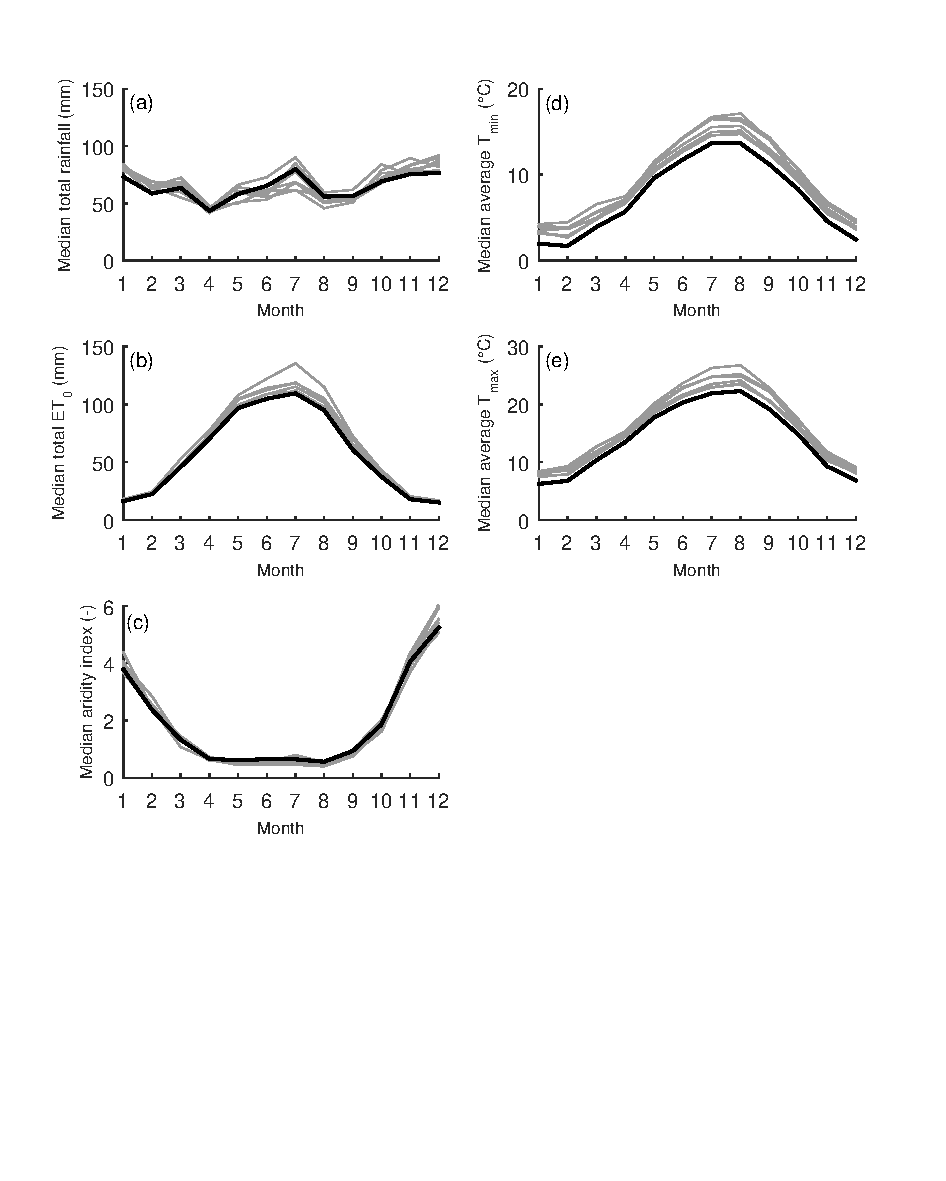
\includegraphics[trim=0.5cm 5.5cm 1.3cm 1cm, clip=true, width=\textwidth]{WeatherGCM_600dpi.pdf}
	\caption{Median (a) total monthly rainfall, (b) total monthly reference evapotranspiration (\ETo), (c) monthly aridity index, (d) monthly average minimum temperature (\Tmin) and (e) monthly average maximum temperature (\Tmax) in the Plankbeek catchment for historical climate of 1985-2014 (black) and  future climate of 2050 as projected by 7 GCMs (grey).}
	\label{fig:ch7_weatherGCM}
\end{figure} 

\begin{table}[!ht]
\setlength{\tabcolsep}{3.2pt}
  \centering
  	\caption{Changes in median annual weather conditions in 2050 as compared to historical weather conditions (1985-2014) for the Plankbeek catchment. The annual aridity index (AI) is the ratio of total annual rainfall over total annual \ETo. Presented range (minimum, median and maximum) for future median changes represent the variety between the median values of each of the 7 GCMs of the ensemble. A positive change value represents an increase, while a negative value represents a decrease.}
\begin{tabular}{lccccc}
\toprule
\multicolumn{2}{l}{\textbf{Annual}} & \textbf{Historical} & \multicolumn{3}{c}{\textbf{Future median change}} \\
\multicolumn{2}{l}{\textbf{weather parameter}}& \multicolumn{1}{c}{\textbf{median}} & \textbf{minimum} & \textbf{median} & \textbf{maximum} \\
\midrule
Total \ETo  & (\si{mm/y}) & 693 & +13   & +51   & +113 \\
Total rainfall  & (\si{mm/y}) & 840 & -9    & +14   & +88 \\
AI & (\si{mm.y/mm.y}) & 1.20 & -0.16 & -0.04 & +0.02 \\
Average \Tmin & (\si{\degreeCelsius})  & 7.4 & +1.0  & +1.8  & +2.5 \\
Average \Tmax & (\si{\degreeCelsius})  & 14.1 & +1.1  & +1.6  & +2.8 \\
\bottomrule
\end{tabular}%
  \label{tab:ch7_WeatherGCM}
  \setlength{\tabcolsep}{6pt}
  \end{table}

\subsubsection{Catchment water availability}
Future annual flow with corresponding subflows is compared to historical conditions in \autoref{fig:ch7_FlowBox} and \autoref{fig:ch7_FlowCDF}. While \autoref{fig:ch7_FlowBox} focuses on presenting variability between the different GCMs of the ensemble and both management scenarios, \autoref{fig:ch7_FlowCDF} also displays inter-annual flow variability. Inter-annual variability is also quantified by means of the flow range (\autoref{tab:ch7_FlowRange}). To complement these visual representations, \autoref{tab:AnB_ChangeQ} lists the exact median annual flow values under historical and future conditions. 

Water availability, represented by the median annual total flow at the catchment outlet, increased under future conditions by 4\% to 27\%. \autoref{fig:ch7_FlowBox} shows that under traditional crop management this increase of total flow (median of 11\%) was caused by an increase of each of the subflows. Median overland flow increased relatively more (12.5\%) compared to interflow (8\%) and baseflow (6\%). However, in absolute terms median baseflow and overland flow increases were almost equal (about \SI{10}{mm/y}). Although variation between different GCMs was rather large, all GCMs pointed towards an increasing flow trend. Only for baseflow and interflow some of the GCMs predicted a small decrease of up to -1\% and -6\% respectively.

On a yearly basis, management adaptations barely affected total flow (\autoref{fig:ch7_FlowBox}). By contrast, the relative contributions to the total flow seriously shifted under adapted management as compared to traditional management. Overland flow strongly reduced (about 20\%) due to implementation of adapted management practices such as tied ridges, while interflow and baseflow increased by 3\% and 8\% respectively. 

Furthermore, apart from median flow also inter-annual flow variability was affected by future conditions (\autoref{fig:ch7_FlowCDF} and \autoref{tab:ch7_FlowRange}). With the exception of interflow, flow variability increased under future climatic conditions. Especially, overland flow became more variable, with a median flow range increase by almost 20\%. Introduction of adapted management, further increased inter-annual variability for baseflow and interflow, but decreased variability for total flow and overland flow as compared to traditional management.

\begin{figure}[tbhp]
	\centering
		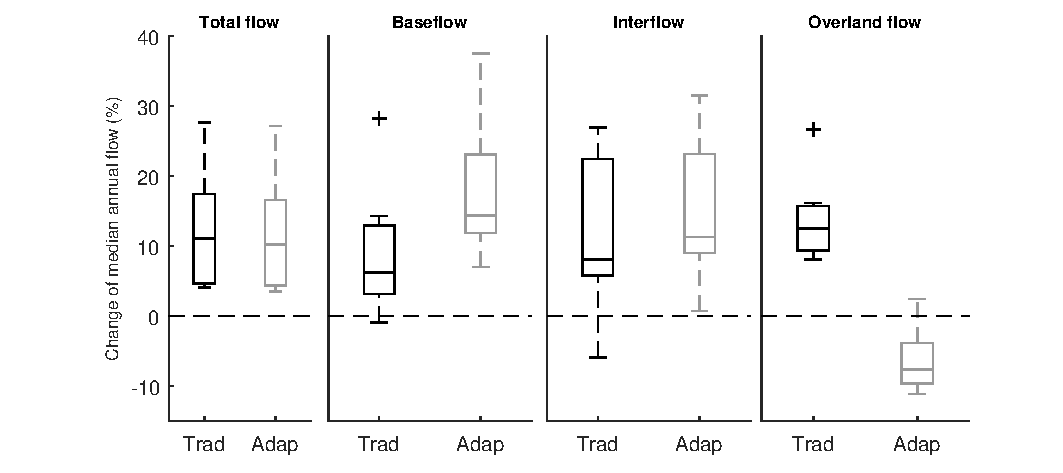
\includegraphics[trim=1.5cm 0cm 1.5cm 0cm, clip=true, width=\textwidth]{FlowBox_600dpi.pdf}
	\caption{Changes of  median annual total flow and subflows in 2050 for the Plankbeek catchment under traditional management (black) and adapted management (grey) with reference to historical conditions (1985-2014). A positive change value represents an increase, while a negative value represents a decrease of annual flow as compared to historical conditions. Boxplots present the variation of the median annual flow change between 7 GCMs.}
	\label{fig:ch7_FlowBox}
\end{figure}  

\begin{figure}[tbhp]
	\centering
		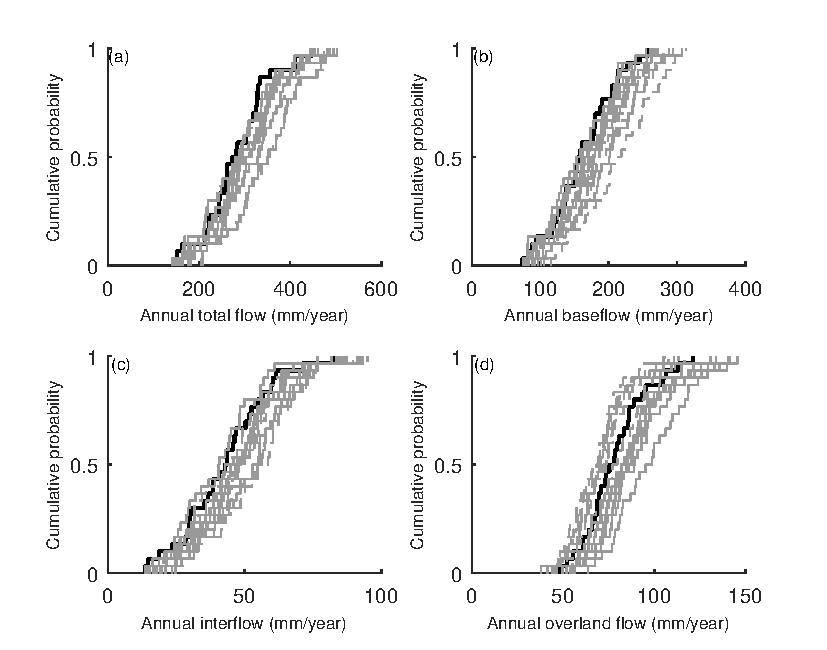
\includegraphics[width=\textwidth]{FlowCDF_600dpi.pdf}
	\caption{Cumulative probability distribution for annual (a) total flow, (b) baseflow, (c) interflow and (d) overland flow under traditional agricultural management in 2050 according to 7 GCMs (grey) as compared to historical conditions (1985-2014) (black). Probabilities were based on 30 seasonal values for the baseline period 1985-2014,  and 30 seasonal values for 2050 for each GCM.}
	\label{fig:ch7_FlowCDF}
\end{figure}   

\begin{table}[htbp]
  \centering
  	\caption{Flow range in 2050 for the Plankbeek catchment under traditional and adapted management as compared to historical conditions (1985-2014). The flow range represents the difference between the maximum and minimum of all annual flow values (n=30). The flow range for future conditions is the median flow range of the 7 GCMs. Values between brackets represent the relative change as compared to historical conditions.}
\begin{tabular}{rcrlrl}
\toprule
 & \textbf{Historical} & \multicolumn{4}{c}{\textbf{Future range (\si{mm/y})}} \\
      & \textbf{range} & \multicolumn{2}{c}{\textbf{Traditional}} & \multicolumn{2}{c}{\textbf{Adapted}} \\
   & \textbf{(\si{mm/y})}&  \multicolumn{2}{c}{\textbf{management}} & \multicolumn{2}{c}{\textbf{management}} \\
\midrule
\multicolumn{1}{l}{Annual total discharge} & 298   & 307   & (+2.9\%) & 303   & (+1.5\%) \\
\multicolumn{1}{l}{Annual baseflow} & 183   & 184   & (+0.4\%) & 190   & (+3.8\%) \\
\multicolumn{1}{l}{Annual interflow} & 69    & 68    & (-0.6\%) & 69    & (+0.6\%) \\
\multicolumn{1}{l}{Annual overland flow} & 73    & 87    & (+19.6\%) & 67    & (-8.1\%) \\
\bottomrule
\end{tabular}%
  \label{tab:ch7_FlowRange}
  \end{table}

Although annual total flow increased for future conditions, this increase of flow is not necessarily spread evenly over the year. To zoom in on seasonal flow changes, \autoref{fig:ch7_FlowMonth} displays changes to the median monthly total flow. 

Changes to total flow as a response to climate change followed the observed weather trends, indicating more arid summers and wetter winters. Median monthly total flow increased during late fall to early spring (November to May), and decreased during summer and beginning of fall. However, \autoref{fig:ch7_FlowMonth} shows large variation between different GCMs. Especially during summer and fall months, for which the GCMs did not even agree whether flow would decrease or increase. Under traditional management,  the median total flow decreased in summer and fall, but some GCMs predicted an increase of total flow. 

Adapted management did not affect median monthly flow much during winter and early spring  months. Between December and April, the difference between both management strategies for median monthly flow was maximum 6\%. By contrast, considering management adaptations makes a large difference in flow predictions (up to 12\%)  for late spring, summer and fall, which corresponds to the growing season of most crops in the catchment. During the main growing season, adapted management increased flow as compared to traditional management. Consequently, the increase of flow in late spring became stronger, while the decrease of flow during summer was counteracted. Only in August adapted management seemed to slightly enforce the decrease of median monthly flow. 

\begin{figure}[tbhp]
	\centering
		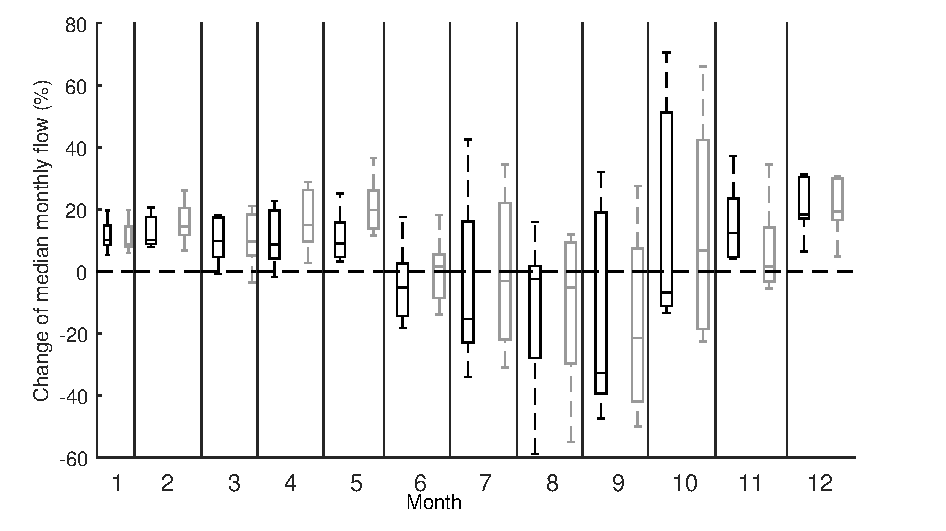
\includegraphics[trim=0cm 0cm 1.5cm 0cm, clip=true,width=\textwidth]{FlowMonth_600dpi.pdf}
	\caption{Changes of  median monthly total flow in 2050 for the Plankbeek catchment under traditional management (black) and adapted management (grey) with reference to historical conditions (1985-2014). A positive change value represents an increase, while a negative value represents a decrease of total flow as compared to historical conditions. Boxplots present the variation of the median monthly flow change between 7 GCMs.}
	\label{fig:ch7_FlowMonth}
\end{figure}   

\subsubsection{Catchment soil water balance and vegetation response}
The observed changes to catchment water availability and various subflows originated from changes to the simulated soil water balance, presented in \autoref{tab:ch7_SWB}. The increase in total flow under future climatic conditions is due to an increase of total rainfall combined with a small decrease of the rainfall fraction that is lost by evapotranspiration. Furthermore, deep percolation and surface runoff increased under future climatic conditions, both in relative and absolute terms, which led to the increase in overland flow as well as interflow and baseflow. Also from the soil water balance it is clear that adapted management decreased surface runoff as compared to traditional management, while deep percolation increased. 

\begin{table}[htbp]
  \centering
  	\caption{Simulated components of the catchment soil water balance in 2050 for the Plankbeek catchment under traditional and adapted management as compared to historical conditions (1985-2014). Positive and negative values present an inflow and outflow over the 30 year simulation period. Water storage includes storage of water in the soil as well as in surface water reservoirs. Values between brackets represent the water flux as a percentage of rainfall. Values for the future are the median flux of the 7 GCMs.}
 \resizebox{\textwidth}{!}{ % minimale correctie om mooi uit te lijnen
\begin{tabular}{lrlrlrl}
\toprule
\textbf{Water} & \multicolumn{2}{c}{\textbf{Historical}} & \multicolumn{4}{c}{\textbf{Future value (mm)}} \\
\textbf{component}   & \multicolumn{2}{c}{\textbf{value (mm)}} & \multicolumn{2}{c}{\textbf{Traditional}} & \multicolumn{2}{c}{\textbf{Adapted}} \\
    & & &  \multicolumn{2}{c}{\textbf{management}} & \multicolumn{2}{c}{\textbf{management}} \\
\midrule
Rainfall & 25042.4 & \multicolumn{1}{l}{(100.0)} & 25801.3 & \multicolumn{1}{l}{(100.0)} & 25801.3 & \multicolumn{1}{l}{(100.0)} \\
Evaporation & -7880.1 & \multicolumn{1}{l}{(-31.5)} & -8541.7 & \multicolumn{1}{l}{(-33.1)} & -8221.8 & \multicolumn{1}{l}{(-31.9)} \\
Transpiration  & -8722.4 & \multicolumn{1}{l}{(-34.8)} & -8091.1 & \multicolumn{1}{l}{(-31.4)} & -8455.8 & \multicolumn{1}{l}{(-32.8)} \\
Deep percolation& -6129.0 & \multicolumn{1}{l}{(-24.5)} & -6511.7 & \multicolumn{1}{l}{(-25.2)} & -6998.9 & \multicolumn{1}{l}{(-27.1)} \\
Surface runoff & -2353.2 & \multicolumn{1}{l}{(-9.4)} & -2620.7 & \multicolumn{1}{l}{(-10.2)} & -2130.2 & \multicolumn{1}{l}{(-8.3)} \\
Net water storage & -66.5 & \multicolumn{1}{l}{(-0.3)} & -66.6 & \multicolumn{1}{l}{(-0.3)} & -66.6 & \multicolumn{1}{l}{(-0.3)} \\
\midrule
Total & -108.8 & \multicolumn{1}{l}{(-0.4)} & -105.8 & \multicolumn{1}{l}{(-0.4)} & -107.0 & \multicolumn{1}{l}{(-0.4)} \\
\bottomrule
\end{tabular}%
}
  \label{tab:ch7_SWB}
  \end{table}

Since \ETo increased and evapotranspiration decreased for future conditions (\autoref{tab:ch7_SWB} and \ref{tab:ch7_WeatherGCM}), the vegetation response to climate change caused a 6.6\% decrease of the evapotranspiration coefficient when evaluated over the whole 30-year simulation period. \KET decreased from 0.79 under historical conditions to 0.74 under future conditions for both traditional and adapted management. \autoref{fig:ch7_kET} shows that these \KET changes were even more pronounced during summer months with median decreases of between 5 to 10\%. For the GFDL-CM3 climate model there was even an increase of about 30\% for August. During fall and winter months, when crop transpiration is limited, the vegetation response to climate change was negligible (\KET decreased by maximum 1\%). Despite the fact that adapted management did not affect \KET when evaluated over the whole simulation period, it clearly affected monthly \KET values. Adapted management partly countered the \KET decrease due to climate change for most months, except for April, May and July.

\begin{figure}[tbhp]
	\centering
		\includegraphics[trim=0cm 0cm 1.5cm 0cm, clip=true,width=\textwidth]{kET_600dpi.pdf}
	\caption{Changes of the median monthly catchment evapotranspiration coefficient (\KET) in 2050 for the Plankbeek catchment under traditional management (black) and adapted management (grey) with reference to historical conditions (1985-2014). A positive change value represents an increase, while a negative value represents a decrease of \KET as compared to historical conditions. Boxplots present the variation of the median monthly \KET change between 7 GCMs.}
	\label{fig:ch7_kET}
\end{figure}   

\subsubsection{Crop yield and water productivity}
Crop yield and water productivity in future as compared to historical conditions is presented in \autoref{fig:ch7_ProdResponse} to \autoref{fig:ch7_ProdCDFMan}. While \autoref{fig:ch7_ProdResponse} presents only the impact of climate and management changes on median crop yield and crop water productivity, \autoref{fig:ch7_ProdCDF} and \autoref{fig:ch7_ProdCDFMan} incorporate inter-annual variability. The latter is also quantified by means the productivity ranges (\autoref{tab:ch7_ProdRange}). Furthermore, \autoref{fig:ch7_ProdCDF} makes it possible to distinguish between the inter-annual variation and variation caused by the different GCMs of the ensemble. Next to these visual representations, \autoref{tab:AnB_ChangeTradMan} and \ref{tab:AnB_ChangeAdapMan} lists the exact median yield and crop water productivity values under historical and future conditions for each crop. 

Median crop yield and water productivity were mostly projected to increase in the future, even without management adaptations. It is very clear from \autoref{fig:ch7_ProdResponse} that both winter wheat and peas benefited most from climatic changes, with a median yield increases of about 22\%. In combination with adapted management, this median yield increase went up to 27\% and 36\% respectively. For maize, the increase of median crop yield was only small (1\%) without adapted management. This could be linked to maize being a C4 crop, which is less responsive to rising \COtwocon as compared to the C3 crops (see \fsink \autoref{tab:ch7_croppar}). Furthermore, it is clear from \autoref{fig:ch7_ProdResponse} that \WPET increased more than crop yield. This indicates that next to an increase of crop yield, seasonal evapotranspiration decreased. 

Although median productivity increased, the crop productivity response differed between the different ensemble GCMs. While winter wheat and peas yield response was clearly positive for all GCMs, yield response for maize, potato and sugar beet was less clear. Median crop yield was projected to increase, but some GCMs predicted a yield decrease of up to 12\% under traditional management and 3\% under adapted management. By contrast, the response for \WPET was never negative. In addition to the fact that GCMs did not agree on the direction of the maize, potato and sugar beet yield response, the variation between different GCMs was also larger for these crops than for winter wheat and peas (\autoref{fig:ch7_ProdResponse} and \autoref{fig:ch7_ProdCDF}). 

Apart from the impact on median crop yield and water productivity, climate change and management adaptations affected inter-annual variability, as seen in \autoref{tab:ch7_ProdRange} and \autoref{fig:ch7_ProdCDF}. It is clear that under future conditions the difference between minimum and maximum productivity increased. Largest range increases were observed for potato yield (up to 27\%) and winter wheat \WPET (up to 74\%) (\autoref{tab:ch7_ProdRange}). Only the maize yield and \WPET range became smaller. 

\begin{table}[htbp]
  \centering
  	\caption{Yield and ET crop water productivity (\WPET) range in 2050 for the Plankbeek catchment under traditional and adapted management as compared to historical conditions (1985-2014). The ranges represent the difference between the maximum and minimum crop yield and \WPET over all simulated seasons (n=30). The range for future conditions is the median range of the 7 GCMs. Values between brackets represent the relative change as compared to historical conditions.}
\begin{tabular}{lcrlrl}
\toprule
\multirow{2}[1]{*}{\textbf{}} & {\textbf{Historical}} & \multicolumn{4}{c}{\textbf{Future range}} \\
      &   {\textbf{range}}    & \multicolumn{2}{c}{\textbf{ Traditional}} & \multicolumn{2}{c}{\textbf{ Adapted}} \\
            &       & \multicolumn{2}{c}{\textbf{ management}} & \multicolumn{2}{c}{\textbf{management}} \\
\midrule
\multicolumn{1}{l}{\textbf{Yield range (\si{t/ha})}} &  &     &       &       &        \\
Maize  & 4.1   & 3.4   &(-15.6\%)& 4.3   & (+5.9\%)\\
Winter wheat  & 4.3   & 4.4   & (+2.2\%)& 4.9   & (+13.2\%) \\
Potato  & 9.5   & 11.6  & (+21.9\%)& 12    & (+26.8\%)\\
Sugar beet  & 5.9   & 6.6   & (+10.8\%)& 7.1   & (+19.3\%) \\
Peas  & 1.9   & 2.3   & (+20.5\%)& 2.2   & (+19.0\%)\\
\midrule
\multicolumn{1}{l}{\textbf{\WPET range (\si{kg/m^3})}} &    &   &       &       &       \\
Maize & 1.5   & 1.1   & (-25.3\%)& 1.3   & (-14.9\%)\\
Winter wheat  & 1.4   & 2.5   & (+74.1\%)& 2.4   & (+69.8\%) \\
Potato & 2.2   & 2.7   & (+21.6\%)& 2.6   & (+18.5\%)\\
Sugar beet & 1.3   & 1.4   & (+8.9\%)& 1.3   & (+3.9\%)\\
Peas  & 0.7   & 0.9   & (+37.3\%)& 0.8   & (+19.8\%)\\
\bottomrule
\end{tabular}%
  \label{tab:ch7_ProdRange}
  \end{table}
 
\begin{figure}[tbhp]
	\centering
		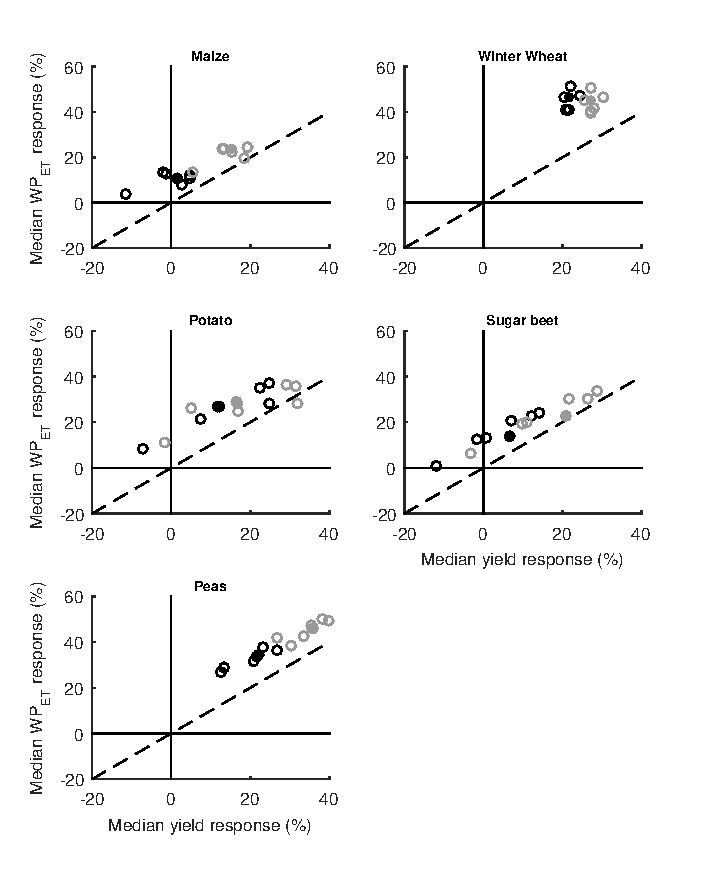
\includegraphics[trim=0cm 0.5cm 1cm 0cm, clip=true,width=\textwidth]{ProdResponse_600dpi.pdf}
	\caption{Changes to median seasonal crop yield and ET crop water productivity (\WPET) for major crops in the Plankbeek catchment under traditional management (black) and adapted management (grey) in 2050 as compared to historical conditions (1985-2014). A positive change value represents an increase, while a negative value represents a decrease of productivity as compared to historical conditions. Open symbols present the median productivity increase of the 7 GCMs, whereas the filled symbol presents the ensemble median.}
	\label{fig:ch7_ProdResponse}
\end{figure}
 
\begin{figure}[tbhp]
	\centering
		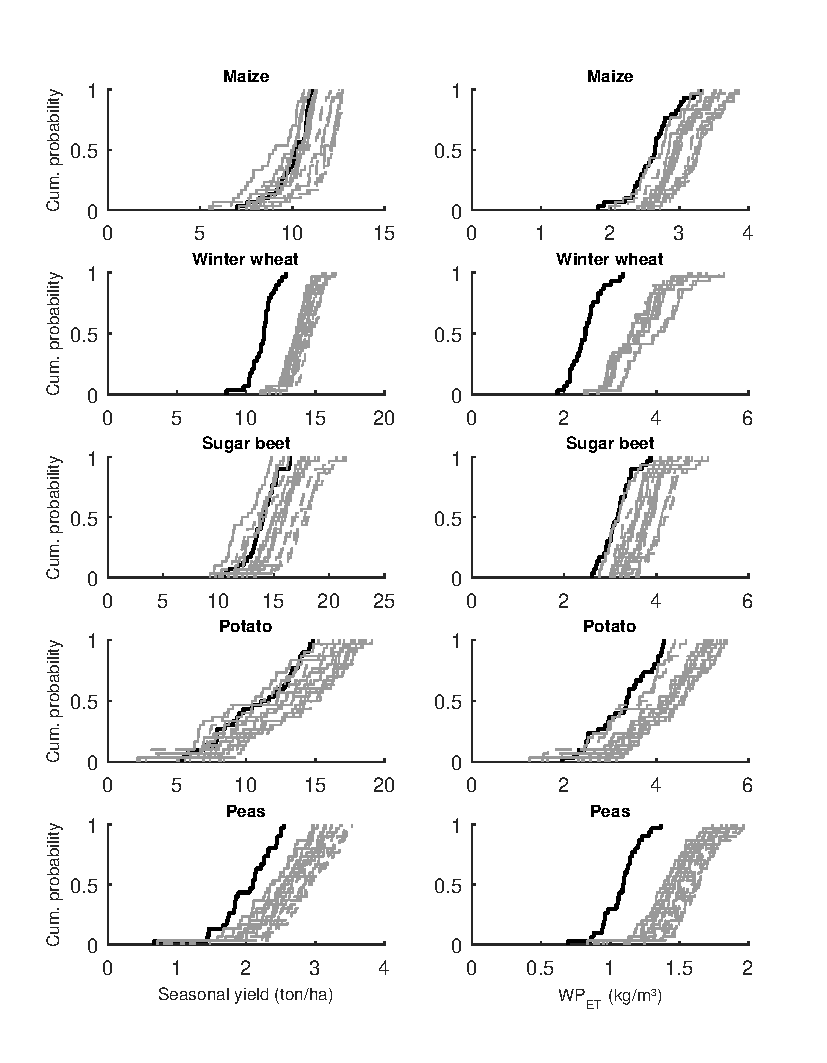
\includegraphics[trim=0.5cm 0.5cm 1cm 0cm, clip=true,width=\textwidth]{ProdCDF_600dpi.pdf}
	\caption{Cumulative probability distribution for seasonal crop yield (left) and ET crop water productivity (right) of major crops in the Plankbeek catchment for historical conditions (black) and future conditions with traditional management according to 7 GCMs (grey). Probabilities were based on 30 seasonal values for the baseline period 1985-2014 and 30 seasonal values for 2050 for each GCM.}
	\label{fig:ch7_ProdCDF}
\end{figure}
\clearpage
Furthermore, \autoref{fig:ch7_ProdCDFMan} clearly indicates that, with the exception of maize and sugarbeet yield, the impact of climate change on productivity was larger than the impact of management adaptations. Nevertheless, the impact of management on crop productivity should not be neglected. Management adaptations ensured that crops could benefit more from the changed climatic conditions, leading to an additional yield increase. This extra yield benefit to adapted management was largest for maize, sugar beet and peas. Although adapted management gave an additional boost to crop yield, it could not reduce yield variability. \autoref{tab:ch7_ProdRange} also shows that for most crops the yield range even further increased when adapted management was considered. Adapted management only stabilized peas yield. 

Finally, \WPET was mostly affected by adaptations of field surface management rather than sowing dates or growing cycle length as indicated by the different \WPET responses of each crop to adapted management (\autoref{fig:ch7_ProdResponse} and \autoref{fig:ch7_ProdCDFMan}). Like yield, largest \WPET responses to management were found for maize, sugar beet and peas. For these crops the field surface adaptations (mulches) strongly reduced evaporation, leading to an increase of \WPET. By contrast, tied ridges did not affect \WPET of potato much. For winter wheat, management adaptations (only growing cycle length) affected \WPET slightly negative. The yield increase due to extension of the growing cycle did not compensate for the extra crop evapotranspiration during the extended growing cycle causing reduction of \WPET. 

\begin{figure}
	\centering
		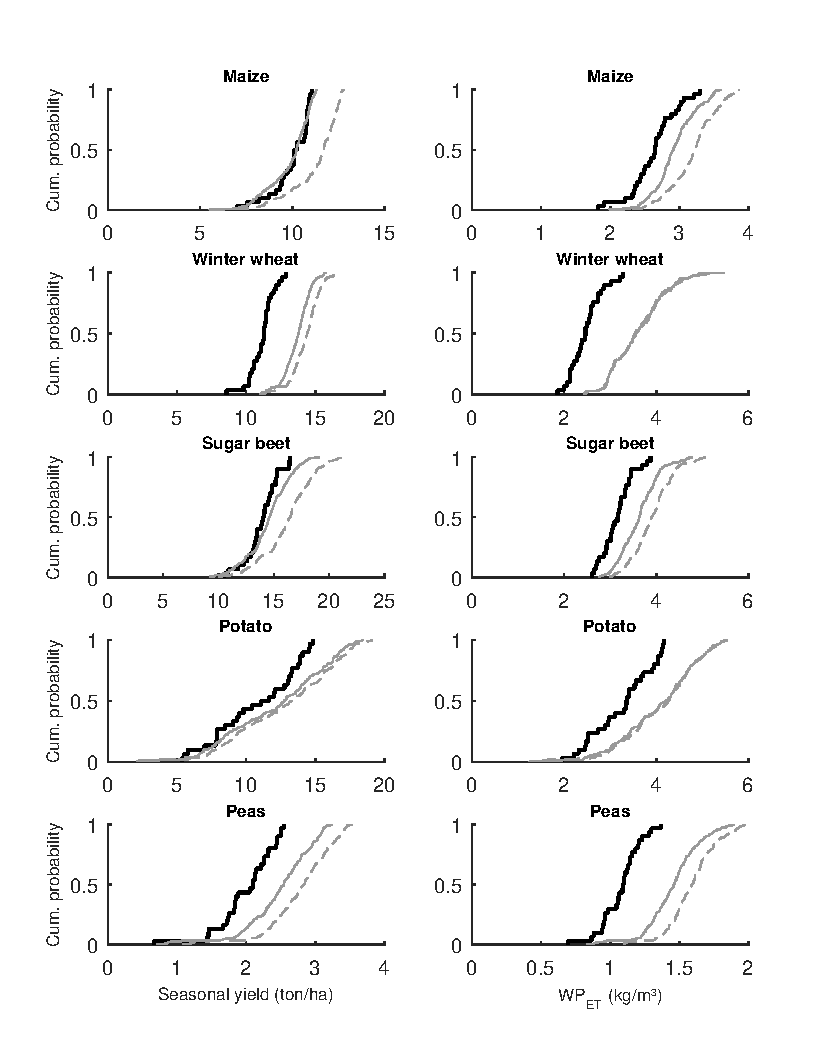
\includegraphics[trim=0.5cm 0.5cm 1cm 0cm, clip=true,width=\textwidth]{ProdCDFMan_600dpi.pdf}
	\caption{Cumulative probability distribution for seasonal crop yield (left) and ET crop water productivity (right) of major crops in the Plankbeek catchment for historical conditions with traditional management (black) and future conditions with traditional (grey full line) or adapted management (grey dotted line). Probabilities were based on 30 seasonal values for the baseline period 1985-2014,  and 210 seasonal values for 2050 representing 30 runs for 7 GCMs.}
	\label{fig:ch7_ProdCDFMan}
\end{figure}

\subsubsection{Length of the growing period}
Due to changes of weather conditions and resulting available soil water, the length of the growing period (LGP) changed under future climatic conditions. \autoref{fig:ch7_LGP} presents the impact of climate and management changes on median LGP. 

Under future climatic conditions the growing period shortened by 5.5 to 25 days. Largest differences were simulated for sugar beet, closely followed by maize and winter wheat (\autoref{fig:ch7_LGP}). This is logical, as those crops also had the longest LGP under historical conditions, and consequently the largest window for LGP reduction. Furthermore, the extension of the growing cycle length and advance of sowing dates under adapted management (\autoref{tab:ch6_Mgmt}) partly compensated for the LGP decrease in the future. 

As LGP is influenced by both temperature and water stress, it is difficult to distinguish which of these factors caused the simulated changes of median LGP that are presented in \autoref{fig:ch7_LGP}. However, the GCMs predicting the largest changes to LGP under future conditions relative to the historical situation (i.e. GFDL-CM3 for spring crops, IPSL-CM5A-LR for winter crops) also corresponded to those predicting the highest temperature increase during the growing season. Hence, it can be assumed that the observed decrease of LGP was mainly caused by increasing temperatures rather than early senescence due to increased water stress. 

\begin{figure}
	\centering
		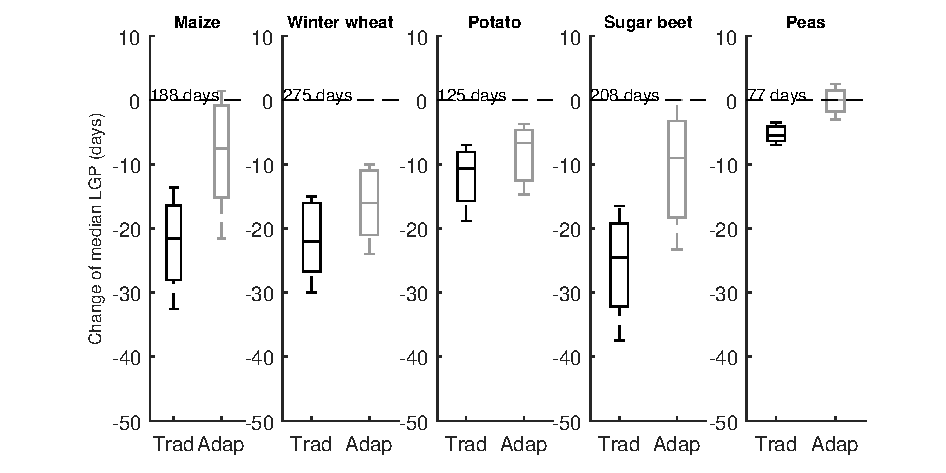
\includegraphics[trim=1.5cm 0cm 1cm 0cm, clip=true, width=\textwidth]{LGP_600dpi.pdf}
	\caption{Change to the median length of the growing period (LGP) of major crops in the Plankbeek catchment under traditional management (black) and adapted management (grey) in 2050 with reference to historical conditions (1985-2014). A positive change value represents an increase, while a negative value represents a decrease of LGP as compared to historical conditions. The historical median LGP is indicated next to the dashed line representing no change. Boxplots present the variation of the median LGP change between 7 GCMs.}
	\label{fig:ch7_LGP}
\end{figure}  

\subsubsection{Water and temperature stress}
Since neither fertility stress nor salinity stress were considered in the simulations, the simulated changes to crop productivity and LGP discussed above can be largely attributed to changes of water and temperature stress (\autoref{fig:ch7_WSI} and \autoref{fig:ch7_CSI}) under future climatic and agronomic conditions. 
 
Under historical conditions, \autoref{fig:ch7_WSI}  shows that water stress decreased crop production most for potato (median WSI 17\%), followed by peas (median WSI 15\%), maize (median WSI 4\%) and sugar beet (median WSI 3\%). By contrast, biomass reduction due to water stress was negligible for winter crops such as winter wheat. Median biomass reduction due to water stress increased due to climate change for potato and sugar beet, as shown in \autoref{fig:ch7_WSI}. For maize and peas the median effect was negligible, but some GCMs predicted an increase of water stress. Furthermore, \autoref{fig:ch7_WSI} shows that adapted management could partly counteract the increase of water-stress, and for maize and peas even improve the situation as compared to historical conditions. By contrast, sugar beet suffered from more water stress  under adapted management. Clearly, mulches could not compensate for the increase of water stress at the end of the season due to longer growing cycles. The effect of water stress on winter wheat production remained negligible in the future, regardless of the management strategy.

\begin{figure}
	\centering
		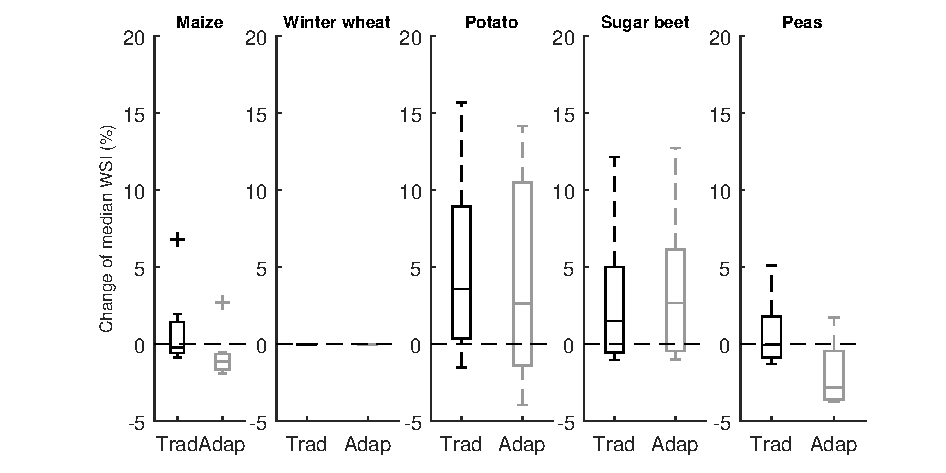
\includegraphics[trim=1.5cm 0cm 1cm 0cm, clip=true,width=\textwidth]{WSI_600dpi.pdf}
	\caption{Changes to median seasonal water stress index (WSI) for major crops in the Plankbeek catchment under traditional management (black) and adapted management (grey) in 2050 with reference to historical conditions (1985-2014). A positive change value represents an increase, while a negative value represents a decrease of the stress index as compared to historical conditions. Boxplots present the variation of the median stress index change between 7 GCMs.}
	\label{fig:ch7_WSI}
\end{figure}   

In addition to water stress, historical crop biomass production was affected by temperature stress.
The seasonal heat stress index (HSI) showed that heat stress affecting pollination did not occur under historical conditions and neither under future climatic conditions. The threshold for heat stress (polmx in \autoref{tab:ch7_croppar}) for summer crops, being \SI{40}{\degreeCelsius}, was only reached on one summer day in 30 year, while the threshold for winter crops (\SI{35}{\degreeCelsius}) was only exceeded outside the flowering period of these crops.

The cold stress index (CSI) in \autoref{fig:ch7_CSI} shows that cold stress was highest for winter wheat (median CSI 33\%). Amongst spring crops, maize (median CSI 31\%) production was most affected by cold stress followed by peas (median CSI 14\%) and sugar beet (median CSI 7\%). Clearly, highest cold stress was experienced by crops that are either very sensitive to cold (e.g. high tb and stbio of maize in \autoref{tab:ch7_croppar}) or have their growing period during colder periods (winter wheat). Potato production was not affected by cold stress under historical conditions, nor under future climatic conditions. For other crops, cold stress decreased due to rising temperatures in the future climate. Largest decreases of cold stress were noticed for winter wheat and maize, with a median CSI decrease of -8\% and -10.5\% respectively.  Hence, largest benefits to the increased temperature were experienced by crops that suffered most from cold temperatures under historical climatic conditions. Finally, due to the changed growing periods under adapted management CSI increased a little bit as compared to traditional management, except for winter wheat for which CSI remained about the same.

\begin{figure}
	\centering
		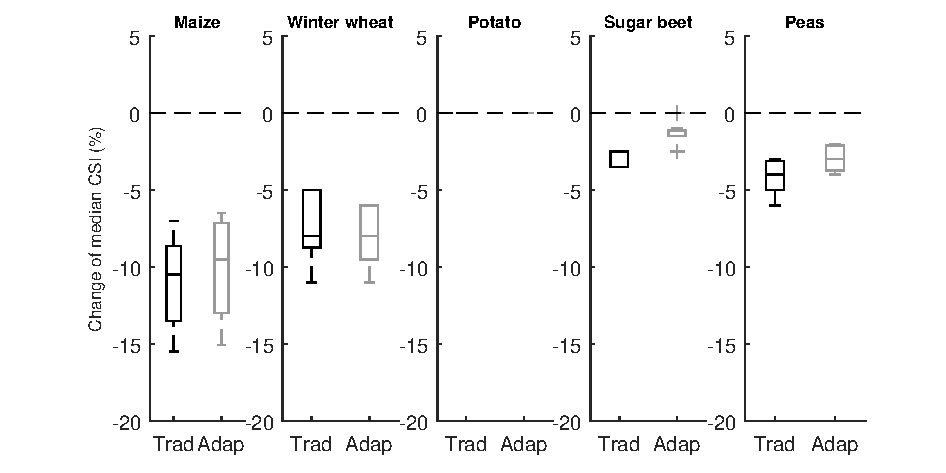
\includegraphics[trim=1.5cm 0cm 1cm 0cm, clip=true,width=\textwidth]{CSI_600dpi.pdf}
	\caption{Changes to median seasonal cold stress index (CSI) for major crops in the Plankbeek catchment under traditional management (black) and adapted management (grey) in 2050 with reference to historical conditions (1985-2014). A positive change value represents an increase, while a negative value represents a decrease of the stress index as compared to historical conditions. Boxplots present the variation of the median stress index change between 7 GCMs.}
	\label{fig:ch7_CSI}
\end{figure}   

\subsubsection{Summary of crop responses to climate and management changes}
Generally, crops in the Plankbeek catchment responded positively to climatic changes, with  simulated median crop yield increasing up to about 22\% and median water productivity increases of up to 46\%. With adapted management, yield increased even up to 36\%. Despite this overall positive picture, the above presented results clearly illustrate how each crop responds differently to climatic changes and related management adaptations. \autoref{tab:ch7_CropSummary} presents a categorical summary of the positive and negative impact on median crop productivity variables and stresses as simulated by AquaCrop-Hydro. 

\begin{table}[htbp]
  \centering
\begin{tabularx}{\textwidth}{p{2.54cm}p{1.4cm}p{1.4cm}p{1.4cm}p{1.4cm}p{1.4cm}}
 	\caption{Impact of climatic change and management adaptations on simulated median crop yield, ET crop water productivity (\WPET), yield range, ET crop water productivity range, length of the growing period (LGP), water stress index (WSI) and cold stress index (CSI). Color codes mark the impact strength. Dark green is a strong positive impact (median change by more than 20\%), green is a moderate positive impact (median change between 5 and 20\%), yellow is a small or negligible impact (median change of maximum 5\%), orange is a moderate negative impact (median change between 5 and 20\%) and red is a strong negative impact (median change by more than 20\%).  Impacts are considered positive when yield or \WPET increase, yield or \WPET ranges decrease, and stress indices decrease.\label{tab:ch7_CropSummary}}\\
\toprule
\multicolumn{1}{c}{\multirow{2}[0]{*}{\textbf{}}} & \multicolumn{1}{c}{\multirow{2}[0]{*}{\textbf{Maize}}} & \multicolumn{1}{c}{\textbf{Winter }} & \multicolumn{1}{c}{\multirow{2}[0]{*}{\textbf{Potato}}} & \multicolumn{1}{c}{\textbf{Sugar}} & \multicolumn{1}{c}{\multirow{2}[0]{*}{\textbf{Peas}}} \\
\multicolumn{1}{c}{} & \multicolumn{1}{c}{} & \multicolumn{1}{c}{\textbf{wheat}} & \multicolumn{1}{c}{} & \multicolumn{1}{c}{\textbf{ beet}} & \multicolumn{1}{c}{} \\
\midrule
\multicolumn{2}{l}{\textbf{Traditional management}} &  &  &  &  \\
Yield & \cellcolor{Yellow} & \cellcolor{Green} & \cellcolor{LimeGreen} & \cellcolor{LimeGreen} & \cellcolor{Green} \\
\WPET  & \cellcolor{LimeGreen} & \cellcolor{Green} & \cellcolor{Green} & \cellcolor{LimeGreen} & \cellcolor{Green} \\
Yield range & \cellcolor{LimeGreen} & \cellcolor{Yellow} & \cellcolor{Red} & \cellcolor{YellowOrange} & \cellcolor{Red} \\
\WPET  range & \cellcolor{Green} & \cellcolor{Red} & \cellcolor{Red} & \cellcolor{YellowOrange} & \cellcolor{Red} \\
WSI   & \cellcolor{LimeGreen} & \cellcolor{Yellow} & \cellcolor{Red} & \cellcolor{Red} & \cellcolor{Yellow} \\
CSI   & \cellcolor{Green} & \cellcolor{Green} & \cellcolor{Yellow} & \cellcolor{Green} & \cellcolor{Green} \\
\midrule
\multicolumn{2}{l}{\textbf{Adapted management}} &  &  &  &  \\
Yield & \cellcolor{LimeGreen} & \cellcolor{Green} & \cellcolor{LimeGreen} & \cellcolor{Green} & \cellcolor{Green} \\
\WPET  & \cellcolor{Green} & \cellcolor{Green} & \cellcolor{Green} & \cellcolor{Green} & \cellcolor{Green} \\
Yield range & \cellcolor{YellowOrange} & \cellcolor{YellowOrange} & \cellcolor{Red} & \cellcolor{YellowOrange} & \cellcolor{YellowOrange} \\
\WPET  range & \cellcolor{LimeGreen} & \cellcolor{Red} & \cellcolor{YellowOrange} & \cellcolor{Yellow} & \cellcolor{YellowOrange} \\
WSI   & \cellcolor{Green} & \cellcolor{Yellow} & \cellcolor{YellowOrange} & \cellcolor{Red} & \cellcolor{LimeGreen} \\
CSI   & \cellcolor{Green} & \cellcolor{Green} & \cellcolor{Yellow} & \cellcolor{Green} & \cellcolor{Green} \\
\bottomrule
\end{tabularx}%
  \end{table}

Under historical conditions, maize biomass production loss due to water stress was limited, while cold stress was rather strong. Water stress mildly decreased and cold stress strongly decreased in future climatic conditions, while heat stress remained absent. The combination of lower stress but a shorter growing period resulted in a negligible difference of median yield. By contrast, \WPET increased and productivity became more stable. Introducing adapted management had a positive effect on water stress and further increased productivity.

Winter wheat suffered negligible production losses due to water stress or heat stress under both historical and future climatic conditions. By contrast, cold stress during cold winter months affected winter wheat production a lot under historical conditions. Under future climatic conditions, cold stress seriously reduced so that winter wheat yield and \WPET strongly increased. However, productivity became also less stable, especially for \WPET. Due to extension of the crop cycle, the yield increase was stronger under adapted management. By contrast, adapted management hardly affected \WPET  as no water saving practices were implemented. 

Potato already suffered from late-season water stress in historical climatic conditions, leading to early senescence and considerable production losses. In addition, this water stress contributed to the high inter-annual productivity variability. Despite the fact that drought stress remained a problem under future climatic conditions, median crop yield increased. It appears that yield increased especially in years with limited water stress, but not in drier years. This led to increased yield variability in future climatic conditions. Implementation of adapted management reduced water stress, and further increased median potato productivity. Neither cold stress nor heat stress was a problem for potato. 

Under historical conditions sugar beet experienced some water stress, especially at the end of the growing cycle. Although water stress increased under future conditions, crop yield and \WPET still increased considerably, especially with adapted management. Unfortunately, also productivity variability increased. Cold stress, which was already rather limited under historical conditions, further reduced under future climatic conditions, while heat stress never affected pollination.

Pea production was already affected by water stress during the canopy expansion phase under historical climatic conditions. In addition, peas also suffered from cold stress due to their rather early sowing date. Under future climatic conditions, water stress did not change much but production was less affected by cold stress. Consequently, yield and water productivity increased very strongly. Under adapted management, water stress could be reduced and productivity increased even more. Unfortunately, also inter-annual variability increased under future conditions, leading to less stable production. Heat stress was absent, as pollination is not considered for legumes such as peas. 
  
\subsection{Climate change impact under synthesized impact scenarios}\label{sec:ch7_synth} 
\subsubsection{Weather conditions}
\autoref{fig:ch7_WeatherSynth} displays the median monthly weather conditions for the four synthesized climate scenarios as compared to future weather conditions projected by the ensemble of 7 GCMs and historical climatic conditions. 

Climate projections for the four scenarios mostly differed during summer and winter months. The high winter scenario (Hw) predicts wetter winters and drier summers, while the high summer scenario (Hs) predicts the opposite. Thereby, drier conditions (low AI) are a combination of a decrease in rainfall and (strong) increase of \ETo, while wetter conditions (high AI) are caused by an increase of rainfall with only a small increase of \ETo. The low scenario (L) is a combination of the two high impact scenarios, as it predicts both winter and summer to be drier. However, the summer is less dry for L as compared to Hw, and winter less dry than for Hs, because \ETo increases were less strong. The mean scenario (M) projections lie in between the high and low scenarios. In fall (September to November) and spring (March to May), all scenarios predicted the same rainfall increase. Also \ETo projections differed not much, except for L which projected a slightly lower \ETo increase in spring and fall months. As a result, spring and fall were wetter for L than for the other scenarios, despite it being the scenario that predicted drier summers and winters. Finally, temperature increases were highest for Hw, and lowest for L for all months. M temperature increases lay in between Hw and L for summer and winter months, but were equal to Hw in spring and fall. Hs resulted in low temperature increases like L, except for winter and spring where temperature increases were equal to M.  

Furthermore, \autoref{fig:ch7_WeatherSynth} shows that the synthesized scenarios predicted similar changes to median monthly weather conditions than the ensemble of GCMs. However, as these synthesized scenarios are based on more GCMs than the 7 selected for these study (\autoref{fig:AppB_PerturbETo}-\ref{fig:AppB_PerturbTemp}), there were some deviations, especially for rainfall and \ETo. It is clear that both winter and summer rainfall fell outside the ensemble range. Moreover, summer \ETo projections for Hs were slightly higher than the highest projections of the ensemble.

\begin{figure}
	\centering
		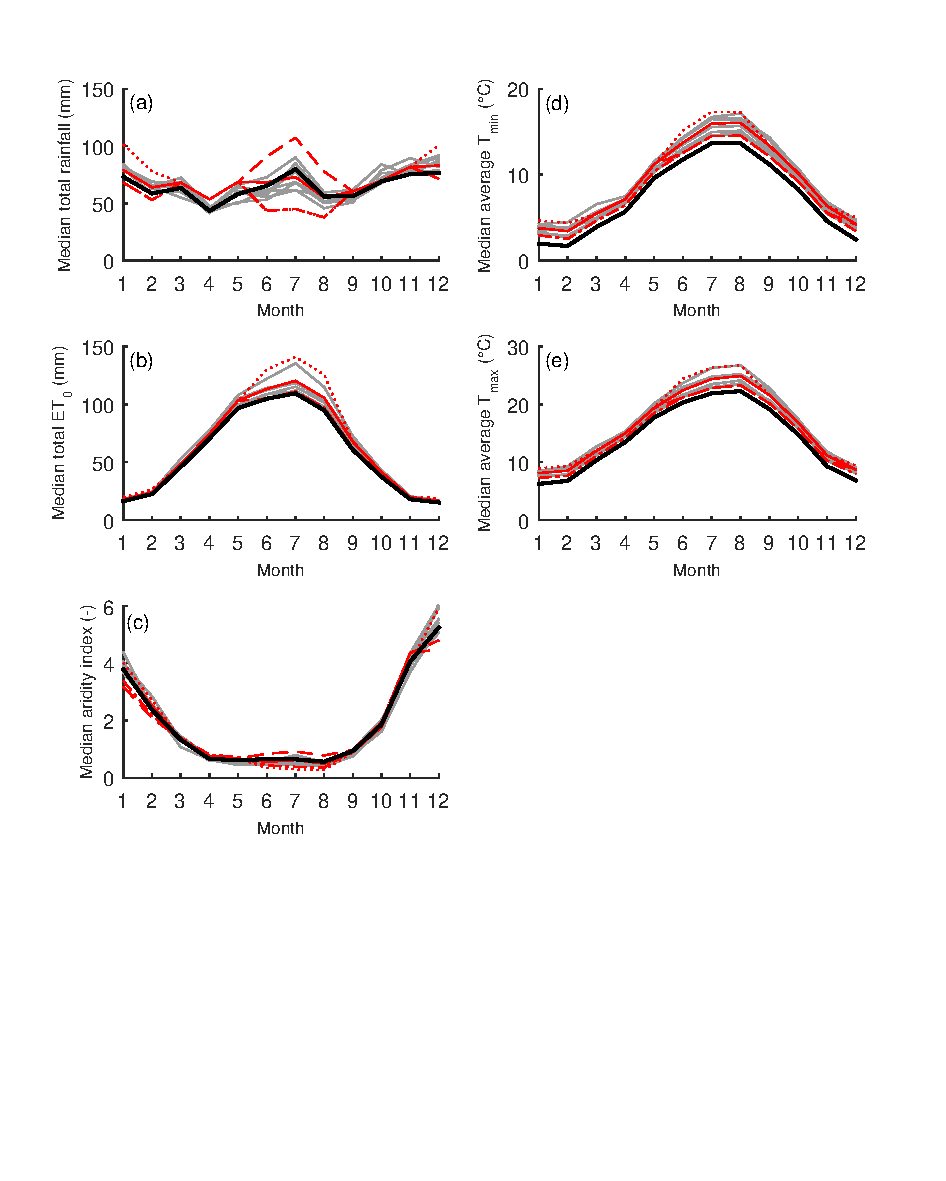
\includegraphics[trim=0.5cm 5.5cm 1.3cm 1cm, clip=true, width=\textwidth] {WeatherSynth_600dpi.pdf}
	\caption{Median (a) total monthly rainfall, (b) total monthly reference evapotranspiration (\ETo), monthly aridity index, (d) monthly average minimum temperature (\Tmin) and (e) monthly average maximum temperature (\Tmax) in the Plankbeek catchment. for historical climate of 1985-2014 (black) and  future climate of 2050 as projected by 7 GCMs (grey) and 4 synthesized scenarios (red). The synthesizeds scenarios correspond to high summer impact  (Hs, dashed red line), high winter impact (Hw, dotted red line), mean impact (M, full red line) and low impact (L, dash-dot red line).}
	\label{fig:ch7_WeatherSynth}
\end{figure}   

\subsubsection{Water availability}
\autoref{fig:ch7_FlowCDFsynth} displays the impact of future weather changes on total flow at the outlet of the Plankbeek catchment, according to simulations with the four synthesized climate scenarios as compared to flow simulated by the ensemble of 7 GCMs or historical time series. 

The simulated changes to total flow at the catchment outlet were completely in line with the simulated weather changes. Hs predicted an increase of total flow in summer, but decrease of flow during winter. For Hw, the opposite was true. Despite their different seasonal effect, annual total flow increased for both high impact scenarios. The annual increase was stronger for Hs than for Hw. L predicted decreasing flow both during summer and winter, so that also annual flow decreased. Finally, M predicted a small increase of both winter and summer flow, as well annual total flow. 

Furthermore, \autoref{fig:ch7_FlowCDFsynth} illustrates that flow projections by the four synthesized scenarios covered a wider range as compared to the ensemble simulations. While the ensemble always projected an increase of annual total flow and winter total flow, L projected a decrease of those flows. Moreover, the increase of summer total flow for Hs was much stronger than any of  the GCMs projections. These deviations between the ensemble and scenarios were clearly related to the deviations of summer and winter rainfall discussed above.

\begin{figure}
	\centering
		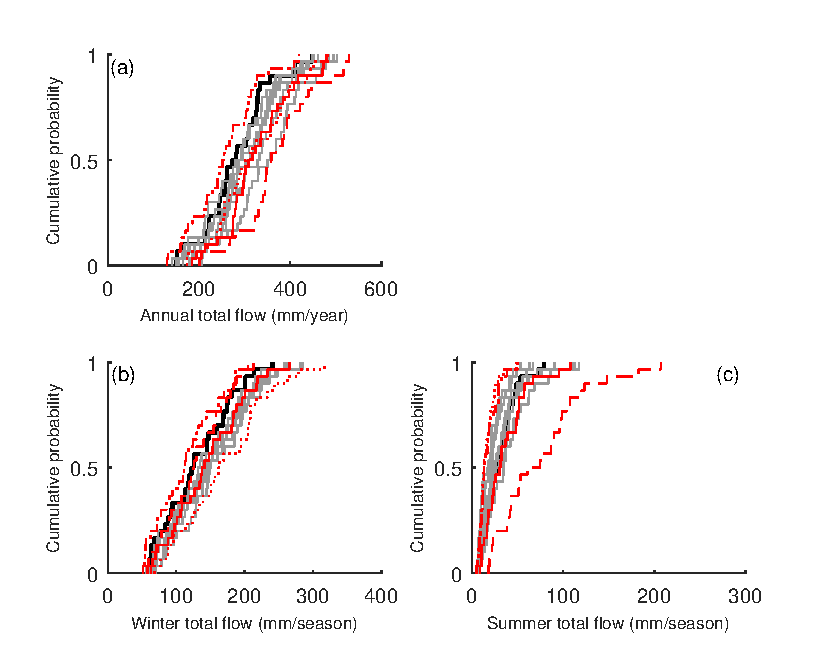
\includegraphics[trim=0.5cm 0cm 1cm 1cm, clip=true,width=\textwidth]{FlowCDFSynth_600dpi.pdf}
	\caption{Cumulative probability distribution for (a) annual (b) winter and (c) summer total flow for historical conditions (black) and future conditions according to the ensemble of climate models (grey) or synthesized scenarios (red): high summer impact (dashed red line), high winter impact (dotted red line), mean impact (full red line) and low impact (dash-dot red line). Probabilities were based on 30 seasons for historical conditions and all synthesized scenarios, but were based on 210 runs for the ensemble of climate models (30 runs for 7 GCMs).}
	\label{fig:ch7_FlowCDFsynth}
\end{figure}   
 
\clearpage
\subsubsection{Crop yield}
\autoref{fig:ch7_ProdBoxSynth} displays the impact of future weather changes on crop yield in the Plankbeek catchment, according to simulations with the four synthesized hydrological impact scenarios as compared to yield simulated by the ensemble of 7 GCMs or historical time series. 

The range of yield impact as simulated by the synthesized scenarios did not match the range of the ensemble simulations. Especially for potato and sugar beet the impact range of the synthesized scenarios was much wider than the ensemble range, while for winter wheat and peas the opposite was true. Only the maize range was about the same. Since also summer rainfall predicted by Hs and Hw fell out of the ensemble range,  it is not surprising that also yield changes for crops grown in summer predicted by Hs and Hw exceeded the ensemble range.   

Furthermore, it is clear from \autoref{fig:ch7_ProdBoxSynth} that the impact predicted by the synthesized scenarios was not consistent amongst crops. Hs corresponded to the highest yield increase for potato, sugar beet and maize, while L resulted in even higher yield increases for peas. For all spring crops Hw resulted in the largest yield decrease or smallest yield increase. For winter crops, such as winter wheat  the opposite is true as Hw caused the largest yield increase. As the dry summers predicted by L were less dry than the dry summers of Hw, L had less negative impact on spring crops than Hw. Moreover, M predictions were only close to the ensemble median for maize and potato. For winter wheat and peas M predicted higher yield increases than the ensemble median, while M gave lower sugar beet yield increases than the ensemble median.

The simulated crop yield impact varied between different crops due to their different sensitivity to temperature and water stress (\autoref{tab:ch7_croppar}), but also because of differences in their timing and length of the growing period (\autoref{tab:ch6_Mgmt}). These differences of the growing period, make that a single scenario can be experienced as a completely different scenario by  each crop. For example, while a winter crop mostly faced wetter winter conditions under Hw, a spring crop was confronted with the drier summer conditions projected by Hw. As a result, large impact differences occurred between winter and spring crops. But, even smaller differences in the growing periods amongst spring crops resulted in different responses to the scenarios. 

Potato and maize (high to low impact : Hs-M-L-Hw), reacted different to the scenarios as compared to peas (high to low impact: L-Hs-M-Hw) and sugar beet (high to low impact : Hs–L-M-Hw). These differences could be linked to earlier planting date (\autoref{tab:ch6_Mgmt}) of sugar beet (15 April) and peas (1 April) as compared to potato and maize (25 April). With earlier sowing, L resulted in a higher yield impact, because it allowed crops to benefit more from the more humid spring conditions predicted by L as compared to other scenarios. This was especially important for peas, which already suffered from water stress in the beginning of the growing season under historical conditions. 

Not only the start but also the length of the growing period seemed to affect the crop yield response to various scenarios. Excluding L, all studied spring crops presented the same order of impact: Hs-M-Hw. This order of decreasing yield impact corresponded to the order of decreasing LGP. Spring crops had a longer LGP under Hs as compared to M and Hw, due to lower temperatures and lower probability of early senescence in the more humid summer of Hs. Since crops can accumulate more biomass and yield with longer growing cycles, it is only logical that yield and LGP impact were linked.  

The LGP – yield response relation worked in the opposite direction for winter wheat. Highest temperature increases under Hw resulted in a short growing cycle, but the highest yield increase. For winter wheat, decrease of cold stress during winter was a stronger determinant for the yield response than the length of the period for building up biomass. 

\begin{figure}
	\centering
		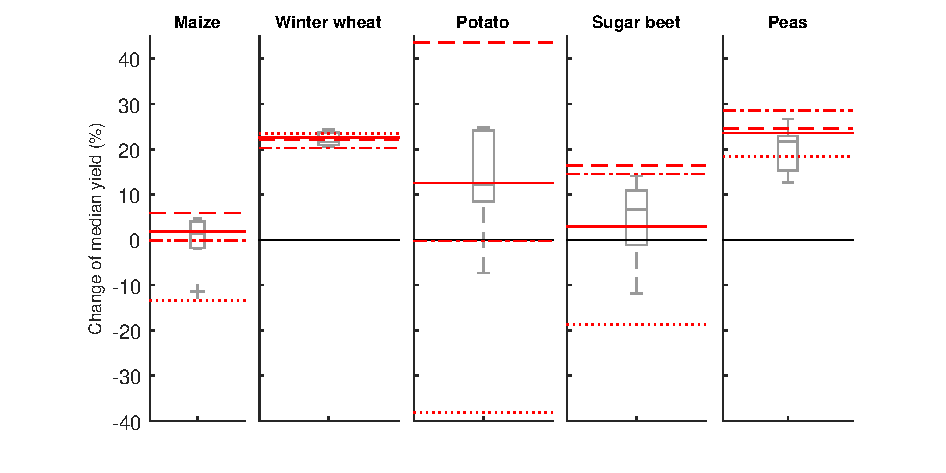
\includegraphics[trim=1.5cm 0.5cm 1.7cm 0cm, clip=true,width=\textwidth]{ProdBoxSynth_600dpi.pdf}
	\caption{Changes to median seasonal crop yield of major crops under traditional management in the Plankbeek catchment in 2050 when simulated by the ensemble of GCMs (boxplots) or synthesized impact scenarios (red lines) with reference to historical conditions (1985-2014). Synthesized scenarios correspond to high summer impact (dashed red line), high winter impact (dotted red line), mean impact (full red line) and low impact (dash-dot red line). A positive change value represents an increase, while a negative value represents a decrease of yield as compared to historical conditions. Boxplots present the variation of the median yield change between 7 GCMs of the ensemble.}
	\label{fig:ch7_ProdBoxSynth}
\end{figure} 
 
\section{Discussion}
\subsection{Impact analysis }
AquaCrop-Hydro shows to be a good tool to simulate the impact of climate change and related management changes for agricultural catchments. This is not surprising as both submodels of AquaCrop-Hydro, i.e. AquaCrop and lumped conceptual models defined according to the VHM approach, were already successfully applied to simulate the impact of climate change on crop production \parencite{vanuytrecht2015, vanuytrecht2014} and catchment hydrology \parencite{vansteenbergen2012, vansteenkiste2012} in Flanders. In addition, it has been shown multiple times that AquaCrop can be used to assess the effect of agricultural management on crop production and the soil water balance (\autoref{ch:aquacrop} to \ref{ch:aquacropscen}).

Obviously, the simulated impact of climate and management changes could not be directly validated with field observations of crop production or discharge in the future. However, the simulated impact matched well with other simulation studies. The simulated changes to catchment water availability are in line with the general projections for late 21\textsuperscript{st} century Belgium by \textcite{tabari2015}. Based on rainfall and reference evapotranspiration projections by an ensemble of CMIP5 climate models, also \textcite{tabari2015}  predicted water availability to decrease in summer but increase in winter. Moreover, the impact on crop yield as simulated by AquaCrop-Hydro is similar to the climate change impact simulated under an ensemble of CMIP3 climate models by \textcite{vanuytrecht2015} for maize, winter wheat, potato and sugar beet cultivated in Flanders on a silt loam soil. Also \textcite{vanuytrecht2015} report a boost to winter wheat, potato and sugar beet yields under future climatic conditions, while maize yield increases are only small. Also management adaptations further boost crop yield for spring crops in the research by \textcite{vanuytrecht2015}, although they report a negligible effect of management on winter wheat production. It should be noted that \textcite{vanuytrecht2015} also used the AquaCrop model for their simulation study (except for winter wheat), so that a good match between results is not surprising. 

By contrast, comparison of the simulated agronomic impact with historical observations of crop yield responses to climatic changes in Europe revealed some inconsistencies. For example, heat stress nor water stress affected winter wheat production in the simulations for the Plankbeek catchment, while \textcite{gouache2015} report that elevated temperatures or excess rainfall during grain filling as well as winter water logging are important variables that explain historical variation of winter wheat yields in 22 French departments. Also \textcite{peltonensainio2010} report harmful effects of elevated temperatures for cereal yield (barley, wheat and maize), based on analysis of the relations between meteorological conditions and crop yield in various European countries including Belgium. Although differences in environmental conditions between these studies and the Plankbeek catchment might partly explain this mismatch between observed and simulated crop responses to climatic changes, also limitations of the AquaCrop-Hydro model seem to be a source of error. 

\subsection{Limitations} 
The simulated impact of climate and management changes was inevitably affected by the design of the impact analysis, the approach to generate future weather data, and AquaCrop-Hydro's model structure and its limitations.

\subsubsection{Impact analysis design}
Because this study only intended to demonstrate application of AquaCrop-Hydro for climate and management impact analysis, certain choices were made to limit the scenario analysis.

First, this study investigated the expected impact for the year 2050 under RCP 8.5. As this scenario projects the highest increase of green house gas emissions, the impact of climate change presented by this study should be seen as a `worst case' scenario for the near future. Clearly, other target years and RCP scenarios would project completely different climate change impacts.

Next, this study considered only one set of potential management adaptations. Although the selected management practices are realistic, more and different adaptations might be implemented in the future. For example, switching crop type, which is also an obvious climate change adaptation strategy, was not considered. Furthermore, it is also expected that farmers will adjust soil fertility management, weed management and crop protection practices in response to altered nutrient cycles and increased incidence of pest and diseases under future climatic conditions \parencite{olesen2011}. Currently, soil fertility management and weed management can be simulated with AquaCrop-Hydro (\autoref{ch:fertility} and \autoref{ch:weed}), but not the occurrence of pest and diseases. Clearly, the simulated impact of agricultural management in this study should merely be seen as an illustration of the potential effect that management could have, rather than as the real management impact that can be expected in the future. 

Finally, this study assessed a limited number of evaluated crops and impact indicators. However, since the selected crops represented 70\% of the total agricultural area and included both winter and spring crops, the results are expected to be representative for the whole catchment. Additional analysis of the climate change impact on grassland would have been interesting, as it covers 18\% of the agricultural area and is an effective erosion control measure. However, the grassland crop parameters could not be validated in \autoref{ch:aquacrophydro} due to lack of data. Consequently, it would be treacherous to focus on the response of grassland to climate and management changes as determined by those parameters.  

\subsubsection{Approach to project future weather conditions}
The most crucial limitation of the impact analysis was the approach that was used to generate future weather data. 

The ensemble approach was affected by the selection of the ensemble composition. Due to limited availability of GCM perturbation signals for minimum and maximum temperature in the perturbation tool, the ensemble existed of only 7 GCMs. A larger ensemble is desired and would increase reliability of the simulated impact range. Moreover, the GCMs of the ensemble originated from only four different research institutes. Since GCMs of the same institute are merely a different parametrization of the same model, it would be better to increase not only the number of GCMs but also diversity of GCMs with respect to their originating institute. Despite the small size and diversity of the selected ensemble, the climatic changes projected by this ensemble match the general trend of changes that was projected by \textcite{tabari2015,tabari2015a} for Belgium using a much larger ensemble of  CMIP5 climate models. 

In addition, sensitivity of model results to the ensemble composition was further investigated by comparison with the climate change impact as simulated using synthesized scenarios. This comparison showed that the synthesized scenarios did not simulate the same impact range as the ensemble of GCMs. The weather, discharge and yield impact range covered by the four scenarios was often larger as compared to the ensemble impact range. This is due to the different number of climate models that was used to obtain perturbation factors for the ensemble and synthesized scenarios. The difference was particularly large for rainfall, with 48 GCMs underlying the synthesized scenarios versus only 7 GCMs included in the ensemble.  Because of the difference in projected rainfall for the future, also the range of simulated discharge and yield impact deviated between the ensemble and synthesized scenarios.

Although also the synthesized scenarios would be more accurate if based on a wider range of climate signals, especially for \Tmin and \Tmax, it is clear that they present a more realistic view on the uncertainty of future climate projections as compared to the limited ensemble. Moreover, they have the advantage that the impact of climate change can be analysed with only few model simulations. This strongly reduces time requirements for data preparation and model simulation. In addition, clearly defined scenarios can facilitate interpretation of the simulated impacts, and thereby improve uptake of information on climate change implications \parencite{wilby2009}.

Despite these advantages, the use of these synthesized scenarios also has its limitations for agro-hydrological impact assessment as demonstrated by this study. Certainly when the scenarios are defined based on their expected hydrological impact and not agronomic impact as done in this study.  On the one hand, the use of hydrologically defined synthesized scenarios worked well to study the impact on river flow at the catchment outlet. The predicted impacts were in line with the expectations under each of the scenarios. Hence, the concern posed by \textcite{ntegeka2014} that scenarios defined according to their expected hydrological impact for a particular catchment in Belgium might not be transferable to other catchments with different locations and properties, was no issue for the Plankbeek catchment. On the other hand, the scenarios did not have a consistent impact on crop production. The synthesized scenarios resulted in different impacts depending on the crop type and timing of the growing period. 

Clearly, this study points out the need to define new synthesized scenarios based on their agronomic impact, either yield or water productivity impact. Defining these synthesized scenarios according to the procedure developed by \textcite{ntegeka2014}, requires many simulations with an agronomic impact model. AquaCrop is a well suited model for this purpose, as it has small calculation times and input requirements. By using AquaCrop-Hydro, one could even consider developing scenarios based on their combined agro-hydrological impact. 

Unfortunately, defining generally applicable agronomic impact scenarios seems extremely difficult. First of all, the impact scenarios would differ for each crop type that has a different growing cycle and sensitivity to climatic changes. This study suggests that for the Belgian conditions a separate set of scenarios for winter and spring crops is the absolute minimum. The results for the Plankbeek catchment indicate that scenarios for winter crops need to be based on the expected temperature changes during the growing season, rather than changes in water availability. A high impact scenario could have a strong increase in temperature, resulting in a strong decrease of cold stress and strong yield increase. Also scenarios for spring crops need to be based on the expected temperature changes during the growing season. But, also changes to water availability should be considered. A high impact scenario for spring crops could represent a small increase in temperature that reduces cold stress while at the same time ensures a long enough growing period, so that final yield increases are strong. In addition, the high impact scenario would need to represent conditions in which crops do not suffer water stress during sensitive periods. As sensitivity to both temperature and water stress is crop (or even cultivar) dependent, scenarios would need to be split up in different categories of spring crops. Second, also other environmental factors complicate development of general agronomic impact scenarios. In particular, soil characteristics and the depth of the groundwater table are highly variable but define water availability to the crop. Hence, scenarios developed based on impact simulations for one soil type are likely not transferable to fields with different soil types. 

Hence, the challenge to define agronomic impact scenarios would be to group cropping systems in such a way that a limited set of scenarios can simulate a consistent impact for all crop and soil types. Only when one succeeds in defining a limited number of agronomic impact scenarios, one could consider development of agro-hydrological impact scenarios. Thereby one needs to deal with the additional complication that various crop combinations are cultivated within the same catchment. 

\subsubsection{Model limitations}
AquaCrop-Hydro has some limitations to study the impact of climate change and related management adaptations, which stem from limitations of its two submodels. 

First, AquaCrop applies highly simplified procedures to simulate the effect of agricultural management such as mulches and tied ridges (\autoref{sec:ch2_Mgmt}). Consequently, some of their potential effects on crop production or the soil water balance are not considered. While mulches reduce soil evaporation, their effect on soil temperature, soil  nutrient status, crop germination and crop development is not directly considered during AquaCrop simulation. In addition, the breakdown of organic mulch material during the growing season is not taken into account. Also the effect of tied-ridges on soil erosion and soil fertility is not considered, because AquaCrop only simulates their inhibition of surface runoff. 

Moreover, AquaCrop considers the effect of heat stress only on pollination or indirectly through increased \ETo (\autoref{sec:ch2_temp}). No direct effect of  heat stress on flowering and grain filling is considered in the AquaCrop simulation procedure. This leads to the unrealistic absence of heat stress for winter wheat and maize simulations. Introducing an adjustment of the harvest index to heat stress, as proposed by \textcite{villalobos2015},  seems indispensable to improve model simulations, especially for future climatic conditions where temperatures are higher. Moreover, due to absence of processes such a cold acclimation, vernalization and dormancy in the AquaCrop simulation procedure, crop response to cold temperatures is simulated less accurately for winter crops. \textcite{vanuytrecht2013} already pointed out that acceptable simulations of winter wheat production under historical conditions could be obtained by adjustment of conservative crop parameters, but that this leads to unrealistic and too strong responses of winter wheat development and production to future temperature increases. In addition, this leads to the wrong impression that winter wheat suffers from cold stress, while this simulated cold stress is merely a technical solution to slow down crop development and biomass production during winter rather than a real stress experienced by the crop. Currently, options to optimize AquaCrop simulation procedures for winter crops are being investigated \parencite{vanuytrecht2014a}. However, as long as model procedures are not updated, AquaCrop should be replaced by more appropriate models, such as the Sirius wheat model \parencite{jamieson1998}, when winter crops are the main interest of the impact analysis or cover a large part of the catchment.

In addition, like other crop models AquaCrop has its limitations to simulate crop response to extreme weather conditions such as droughts, heavy precipitation, heat waves, extreme cold, wind and hail storms. However, the incidence of such extreme weather conditions, which seriously impact crop production and water availability, is likely to increase due to climate change \parencite{ipcc2014}. Currently, options to improve model simulation of crop response to extreme weather conditions is being investigated in the framework of the MODEXTREME (MOdelling vegetation responses to EXTREMe Events) project \parencite{villalobos2015}. 

Second, also the water routing model has some limitations due to its conceptual nature. Because of lack of observations for the future, it is impossible to calibrate the hydrological parameters to match the future catchment response behaviour. Consequently, for this impact analysis the same set of hydrological model parameters was used for all model simulation. These parameters were calibrated and validated for historical conditions in \autoref{ch:aquacrophydro}.  When using the same set for future conditions, it is assumed that neither management changes nor vegetation changes in response to climate change would affect catchment hydrological behaviour. However, in reality field management adaptations such as tied ridges and mulches might affect overland flow recession time. Also denser canopy cover, as a result of more favourable climatic conditions for crop growth, could affect water routing. Nevertheless, the use of fixed recession constants is common practice in hydrological climate change impact assessment. Amongst others \textcite{taye2011} and \textcite{vansteenbergen2012} used fixed model parameters for climate change impact assessment with VHM-type conceptual models. 

\subsection{Implications} 
Many lumped conceptual hydrological models could have been used to study the impact of climate change on runoff at the outlet of the Plankbeek catchment. However, AquaCrop-Hydro has the advantage of being more dynamic with respect to the catchment's response behaviour to climatic changes. The soil water balance simulations of conceptual hydrological models under climate change are only affected by changes in input of rainfall and potential evapotranspiration, but not by changes to vegetation in the catchment. The relation between actual and potential evapotranspiration remains unaffected by climate change, expect for the soil water balance correction. Consequently, vegetation feedbacks to the hydrological system are completely neglected. By contrast, AquaCrop-Hydro simulates actual evapotranspiration not just based on climatic conditions (\ETo) and the soil water balance, but also based on the simulated crop canopy development. Hence, when climate change causes alterations to the canopy structure, the simulated evapotranspiration will be automatically adjusted. This research showed that the catchment's evapotranspiration coefficient decreased by up to 10\% during summer months for future climatic conditions. Since about 65\% of the rainfall in the Plankbeek catchment does not reach the river but is lost by evapotranspiration, conceptual hydrological models make a considerable error when neglecting the vegetation responses to climate change. Especially for accurate simulation of water availability during summer months it is crucial to use a dynamic equation for estimation of evapotranspiration. \textcite{vanwalsum2012} already stressed that a static approach like adopted by conceptual hydrological models should be abandoned in favour of a dynamic approach. AquaCrop-Hydro provides an opportunity to do so, without forcing people to switch to complex physically based models with high data and calibration requirements.

Furthermore, this study highlighted the importance of taking into account management changes for climate change impact assessment. Yield increases due to climate change were up to 14\% higher with adapted management as compared to traditional management. Although total flow was not affected much by management on a yearly basis, flow during late spring, summer and fall was strongly affected by agricultural management practices. Moreover, also the contributions of different subflows to total river discharge were affected by management. This clearly indicates that it is dangerous to neglect the agricultural management aspect when assessing the impact of climate change for agricultural areas. Nevertheless, an analysis of 221 peer reviewed studies on simulation of crop response to climate change showed that only 75\% considered management adaptations, with only 33\% varying at least two management practices.  

Unfortunately, while climate change projections are widely available, projections for future management are sparse. It is extremely difficult to predict management changes for the future, because management is not just affected by environmental factors but also by factors such as farmers' behaviour, legislation and technology advances. For that reason, published information is sparse, mostly based on extrapolation of historical trends, considers few crops, studies one management practice at the same time, and links changes of this management practice just to one determinant factor. For example, this study relied on changes of the planting date based on projected temperature changes. Thereby, the effect of soil wetness and field accessibility on the planting date was not considered. Moreover, a holistic projection of changes to the combination of planting date, growing cycle length and surface practices was absent. Clearly, also AquaCrop-Hydro remains liable to the lack of projections of future agricultural management. Seeing that management can have such a large impact, development of holistic management scenarios deems indispensable. Moreover, an ensemble of such scenarios should be considered due to the high uncertainty related to farmers management decisions.
 
In addition to this lack of information, agricultural management is often disregarded in hydrological impact assessments because of model restrictions. On the one hand, conceptual models cannot explicitly take into account management changes due to lack of physically based model equations and parameters. On the other hand, accurate parametrization to consider management practices is often neglected in physically based models, due to restrictions of data or time for data preparation and model simulation. Fortunately, AquaCrop-Hydro facilitates consideration of agricultural management practices in climate change impact assessment, as simulation of management practices requires few input parameters that are easily available. 

Besides the benefit of a dynamic and realistic simulation of the climate change impact with AquaCrop-Hydro, the impact can be analysed on different scales. AquaCrop-Hydro allows to study the impact of climate change both on agricultural production at field scale as well as catchment water availability. Such a combined analysis is rarely done, but crucial nevertheless. As shown by this study, agricultural management can have a large impact on seasonal water availability in the area, where different actors share the available water resources. Furthermore, also feasibility of climate change adaptations for improving agricultural productivity are often highly dependent on water availability. For example, farmers could benefit more from higher yield due to climate change when the effect of drought stress during summer would be avoided by irrigation. However, shifting from rainfed to irrigated agriculture is only feasible when sufficient irrigation water is available. This study already indicated that supplemental irrigation using river water in the Plankbeek catchment would prove difficult as river flows during summer also decreased due to climate change.

\section{Conclusion}
AquaCrop-Hydro enables simulation of the impact of climate change and related adaptation management strategies on crop production as well as catchment water availability, without large data and calibration requirements. However, further development of AquaCrop is necessary to improve the simulation of crop responses to temperature and extreme events. Because of AquaCrop-Hydro's dynamic nature and the possibility to include the effect of agricultural management, it is expected that its impact projections are more realistic than those of static conceptual hydrological models which cannot take into account management adaptations. Using synthesized climate scenarios can facilitate climate change impact assessment with AquaCrop-Hydro, and avoid biased uncertainty analysis by using a small ensemble of climate models. However, new synthesized climate scenarios that focus on the agronomic impact in addition to the hydrological impact of climate change need to be developed.   


\cleardoublepage